\documentclass[a4paper,10pt,notitlepage]{scrreprt}

\usepackage[T1]{fontenc}
\usepackage[english]{babel}
\usepackage[utf8x]{inputenc}
\usepackage{setspace}
\usepackage{subfig}
\usepackage{textcomp}
\usepackage{graphicx}
\usepackage{fixltx2e}
\usepackage{multirow}
\usepackage{array}
\usepackage{amssymb}
\usepackage{amsmath}
\usepackage{subfig}
\usepackage{nomencl}
\usepackage[pdfborder={0 0 0}]{hyperref}
\usepackage{natbib}
% \usepackage{makeidx}
\usepackage{nicefrac}
\usepackage{bbold}

\captionsetup{labelfont=footnotesize,textfont=footnotesize}

\newcolumntype{x}[1]{>{\begin{flushleft}$}p{#1}<{$\end{flushleft}}}
\newcolumntype{y}[1]{>{\begin{center}$}p{#1}<{$\end{center}}}
\newcolumntype{z}[1]{>{\begin{flushright}$}p{#1}<{$\end{flushright}}}
\newcolumntype{m}{>{$}l<{$}}
\newcolumntype{n}{>{$}c<{$}}
\newcolumntype{o}{>{$}r<{$}}

\newcommand{\mat}[1]{\mathbf{#1}} 

\bibliographystyle{plain}

% Title Page
\title{Scientific Visualization\\Project II}
\author{Milian Wolff}


\begin{document}
\maketitle

\begin{abstract}
Our second project in the scientific visualization class by Eugene Zhang gave
us the opportunity to get acquainted with the algorithms behind ``pen-and-ink
sketching'' of a 3D mesh surface. First we explore the steps required to
visualize silhouettes of a geometry. Then we calculate the vertex-based
curvature and curvature tensors. Finally we will combine the both to draw a
sketch-like version of a given geometry.

The source code of my exercise solutions can be found online under

\begin{center}\url{https://github.com/milianw/scivi}\end{center}
\end{abstract}

\begingroup
\let\clearpage\relax

\tableofcontents
\endgroup

\chapter{Corner Table}

As a foundation for the later tasks we first had to implement a corner table. I
did this by following the steps outlined in class:

\begin{itemize}
 \item iterate over all triangles
 \item add each corner in the triangle to a table
 \item sort table by $min(c.prev.vertex, c.next.vertex)$ and
$max(c.prev.vertex, c.next.vertex)$
 \item iterate over sorted table and associate consecutive rows with equal
$min$ and $max$ entries as opposite corners
\end{itemize}

The implementation can be found in \texttt{CornerTable.java}.

The resulting corner table is essentially a linked list which is straight
forward to use. I additionally added a \texttt{Corner[] vertexNeighbors()}
method to my \texttt{Corner} object, which essentially returns the 1-ring
vertex neighbors.

\section{Validation}

To verify the correctness of my implementation of a corner table, I wrote
\texttt{Ex2\_1.java}. When started, the user defines a geometry. Then the corner
table for said geometry is computed. Now we iterate over each corner \texttt{c}
and run a set of assertion-based tests in each step:

\begin{itemize}
 \item \texttt{c.next != null}
 \item \texttt{c.prev != null}
 \item \texttt{c.next.triangle != c.triangle}
 \item \texttt{c.prev.triangle != c.triangle}
\end{itemize}

Furthermore, the correctness of the ``opposite''-association is validated by
asserting the following tests:

\begin{itemize}
 \item \texttt{c.triangle != c.opposite.triangle}
 \item \texttt{c.next.vertex == c.opposite.prev.vertex}
 \item \texttt{c.prev.vertex == c.opposite.next.vertex}
 \item \texttt{c == c.opposite.opposite}
 \item \texttt{c.prev.opposite.next.vertex == c.next.vertex}
 \item \texttt{c.prev.opposite != c.next}
 \item \texttt{c.prev.opposite.prev.vertex == c.vertex}
 \item \texttt{c.prev.opposite.prev != c}
 \item \texttt{c.next.opposite.prev.vertex == c.prev.vertex}
 \item \texttt{c.next.opposite.prev != c.prev}
 \item \texttt{c.next.opposite.next.vertex == c.vertex}
 \item \texttt{c.next.opposite.next != c}
\end{itemize}

Keep in mind though that in open surfaces like e.g. \texttt{Gauss\_3042.byu} not
every corner can be associated to an opposite one. This is handled gracefully in
my corner table implementation and unit tests.

Another implicit verification of my implication lies in the extensive usage of
the corner table in the following exercises. Since the solutions there seem to
be visually correct, the corner table seems to yield correct results.

\chapter{Silhouette}

Now we want to find the silhouette of a 3D geometry using two different
algorithsm. My solutions to both can be found in \texttt{Silhouette.java} and
\texttt{Ex2\_2.java}.

\section{Face-based approach}

The first task was to find the silhouette by iterating over all edges and
finding those, where only one of the adjacent triangles is ``visible''. Here, we
consider a triangle $T$ to be visible when

\begin{equation}
 (\vec{c}_T - \vec{v}) \cdot \vec{n}_T < 0,
\end{equation}

with $\vec{c}_T$ being the center and $\vec{n}_T$ being the normal of the
triangle respectively. $\vec{v}$ is the position of the viewer.

Note that this approach yields undefined results for triangles that are
exactly perpendicular to the view ray. There, the dot product will be zero and
the triangle is either an invisible backside or a visible frontside. I ignore
these edges, assuming that this case only happens for faces somewhere in the
middle of the (in-)visible surface and are thus not part of the silhouette
anyways.

Now to actually find the silhouette, I first iterate over all triangles and
store the associated index to a list $L$ when the triangle is visible. Then
I iterate over the corner table and find corners $c$ within a visible triangle,
i.e. $c.triangle$ is contained in $L$. Then the edge between $c.prev.vertex$
and $c.next.vertex$ is part of the silhouette, if either $c.opposite$ is
undefined, or alternatively $c.opposite.triangle$ is not contained in $L$.

My implementation of the above can be found in
\texttt{Silhouette.createFaceBasedSilhouette()}.

\subsection{Problems}

The silhouette is view dependendend and \texttt{Ex2\_2} hence recalculates the
silhouette whenever the view point changes. Now when rotating a given geometry,
the main problem of this approach becomes apparent: Gradual changes in the view
can have a big difference one the silhouette. Comparing e.g. fig.
\ref{fig:face-silhouette-bunny-1} and \ref{fig:face-silhouette-bunny-2} shows
this issue at the right ear. Additionally we also see three artifacts, two on
the body and one at the left eye.

The same issue is also responsible for the jagged edge of the sphere silhouette
as visible in fig. \ref{fig:face-silhouette-sphere}. 

\begin{figure}
  \subfloat[]{
    \label{fig:face-silhouette-bunny-1}
    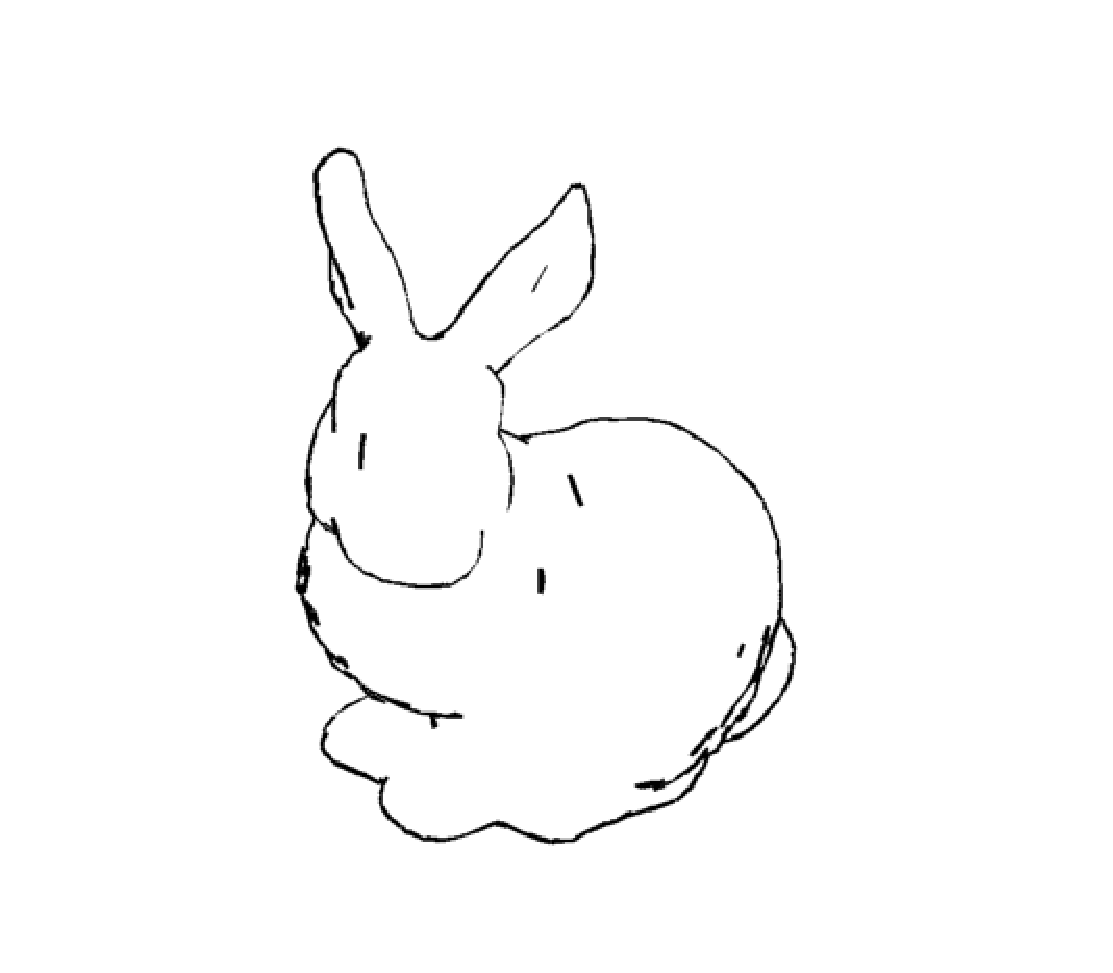
\includegraphics[scale=0.35]{img-2-2/bunny-1.eps}}
  \subfloat[]{
    \label{fig:face-silhouette-bunny-2}
    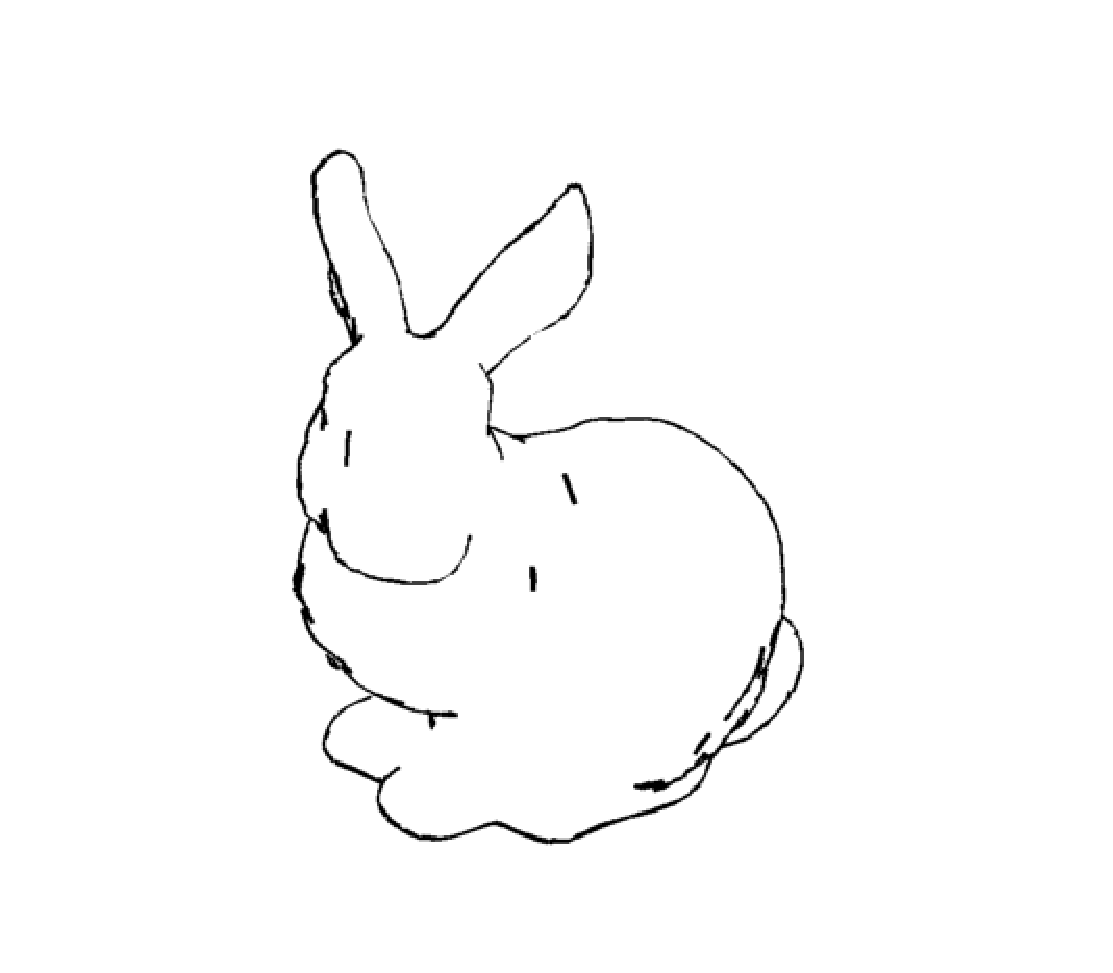
\includegraphics[scale=0.35]{img-2-2/bunny-2.eps}}
 \caption{Face-based silhouette of the bunny under slight rotation}
 \label{fig:face-silhouette-bunny}
\end{figure}

\section{Vertex-based approach / zero level set}

In an attempt to fix the issues of our first approach, we now apply a different
scheme that computes the so called zero level set. That is the curve on the
surface where the dot product between the curve normal and the view ray is
always zero.

To compute this curve we iterate over the corner table and calculate the dot
product between the view ray and the normal at the corner vertex $c$ and its
previous and next vertex $p$ and $n$:

\begin{eqnarray}
 d_{c} = a = (\vec{c} - \vec{v}) \cdot \vec{n}_c \\
 d_{p} = b = (\vec{p} - \vec{v}) \cdot \vec{n}_p \\
 d_{n} = c = (\vec{n} - \vec{v}) \cdot \vec{n}_n
\end{eqnarray}

If we then encounter a triangle where either $a \leq 0$, $b \geq 0$ and $c \geq
0$ or $a \geq 0$, $b \leq 0$ and $c \leq 0$, then a zero level set line goes
through this triangle. We assume it can be approximated
linearly interpolating $a$ and $b$ onto the edge between $c$ and $p$ and
analogously for $a$ and $c$ and then connecting the two points for which the
interpolated dot product should yield zero.

The code for my implementation can be found in
\texttt{Silhouette.createVertexBasedSilhouette()} and
\texttt{Silhouette.findZeroLevel()}.

\subsection{Comparison}

The vertex-based silhouette yields mostly better results, as can be seen in
e.g. figs. \ref{fig:silhouette-sphere}, \ref{fig:silhouette-dragon},
\ref{fig:face-silhouette-feline} or \ref{fig:face-silhouette-buddha}.

Personally I find the comparison between the two algorithms as
applied to the dragon in fig. \ref{fig:silhouette-dragon} and the feline in fig.
\ref{fig:face-silhouette-feline} the most interesting. While in both cases, the
vertex-based approach yields subjectively more correct silhouettes, the
face-based approach yields a visually more pleasing result for the silhouette
in fig. \ref{fig:face-silhouette-feline}. Here the rendering artifacts, that
look bad in the dragon, actually make the image more detailed and hence more
similar to an actual ``pen-and-ink'' scetch. The same happens for the buddha in
\ref{fig:face-silhouette-buddha}.

\begin{figure}
  \subfloat[face-based]{
    \label{fig:face-silhouette-sphere}
    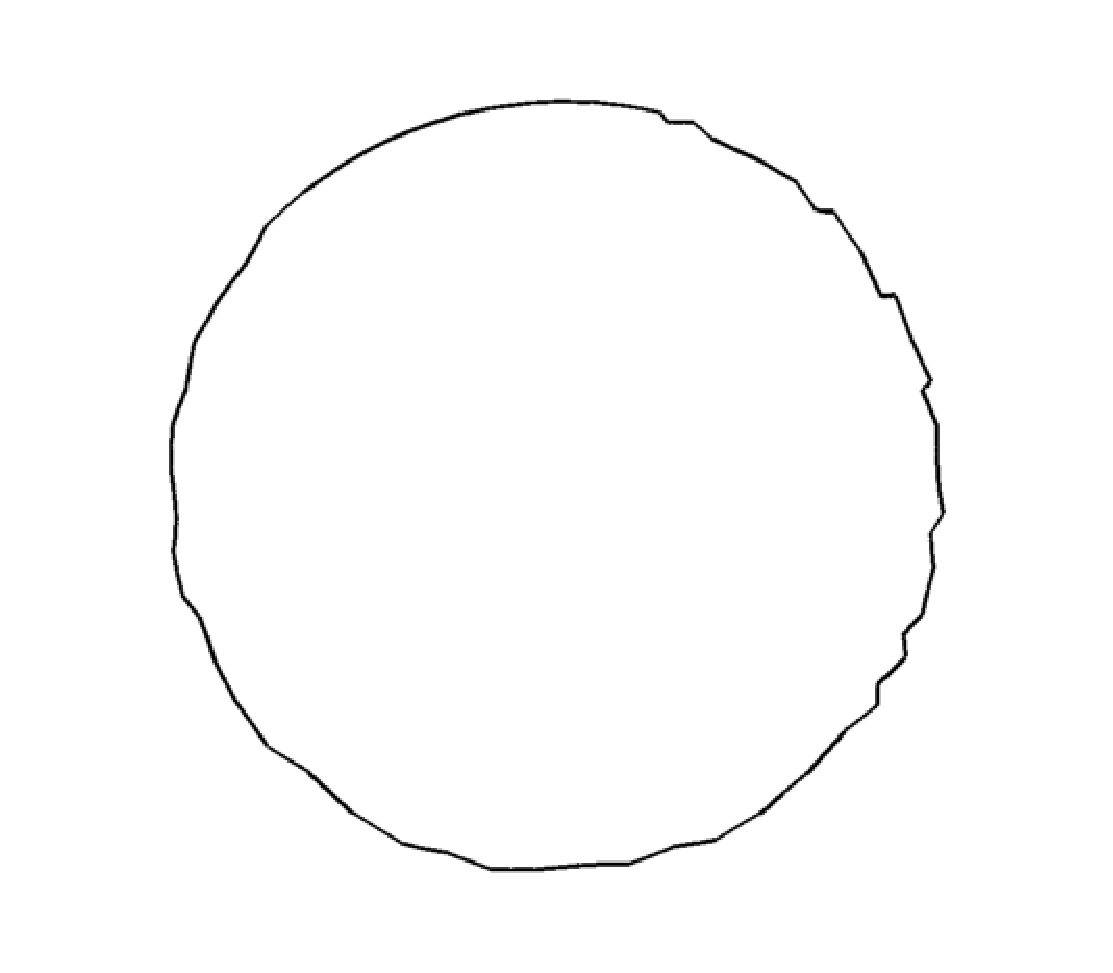
\includegraphics[scale=0.35]{img-2-2/sphere-face.eps}}
  \subfloat[vertex-based]{
    \label{fig:vertex-silhouette-sphere}
    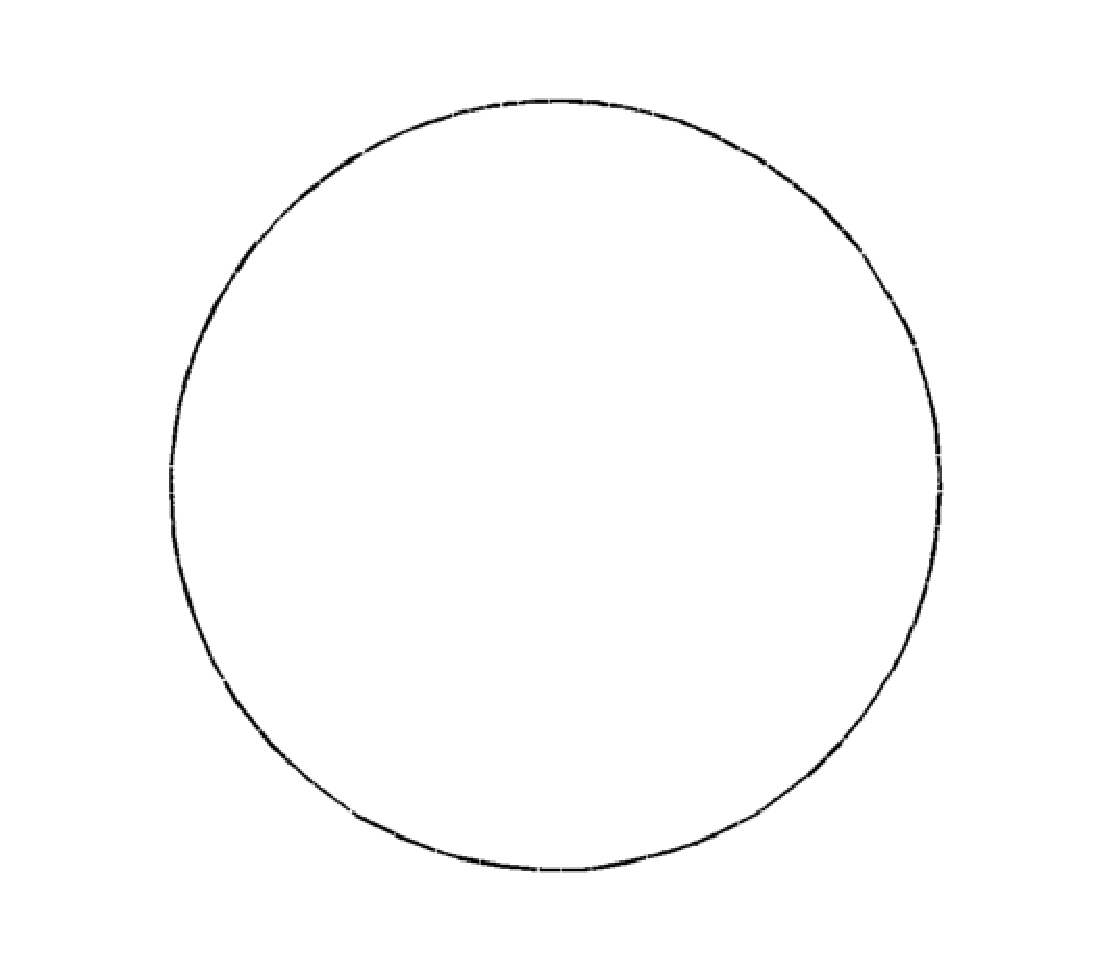
\includegraphics[scale=0.35]{img-2-2/sphere-vertex.eps}}
 \caption{Comparison of face- and vertex-based silhouette for the sphere}
 \label{fig:silhouette-sphere}
\end{figure}

\begin{figure}
  \subfloat[face-based]{
    \label{fig:face-silhouette-dragon}
    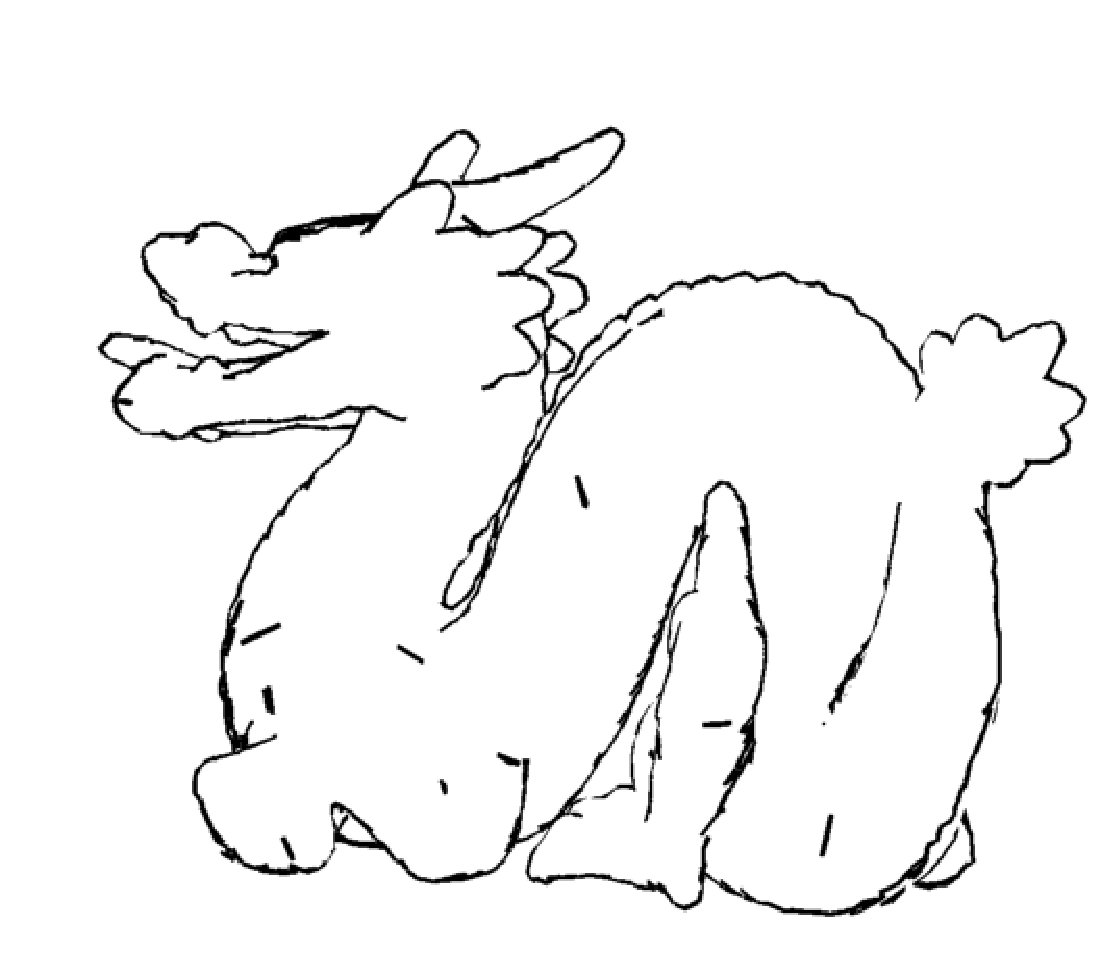
\includegraphics[scale=0.35]{img-2-2/dragon-face.eps}}
  \subfloat[vertex-based]{
    \label{fig:vertex-silhouette-dragon}
    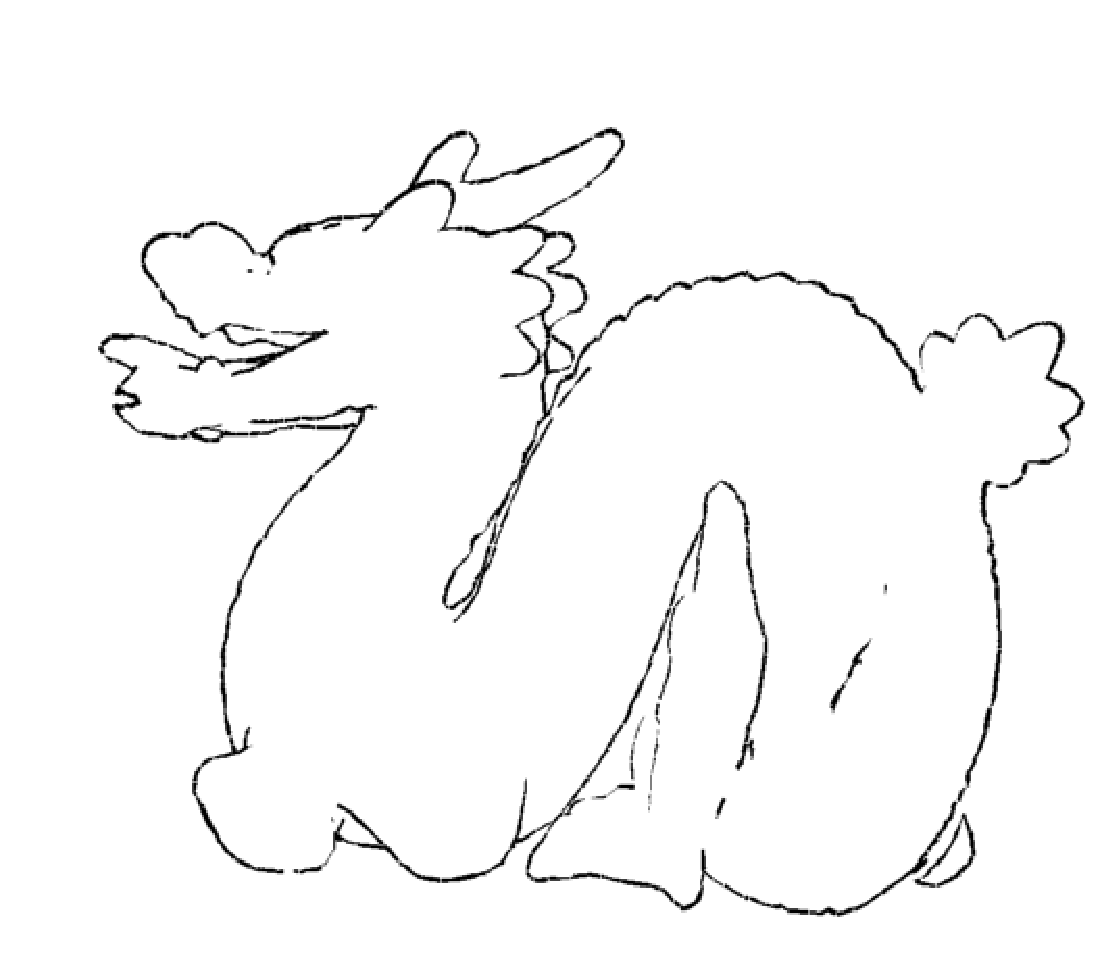
\includegraphics[scale=0.35]{img-2-2/dragon-vertex.eps}}
 \caption{Comparison of face- and vertex-based silhouette for the dragon}
 \label{fig:silhouette-dragon}
\end{figure}

\begin{figure}
  \subfloat[face-based]{
    \label{fig:face-silhouette-feline}
    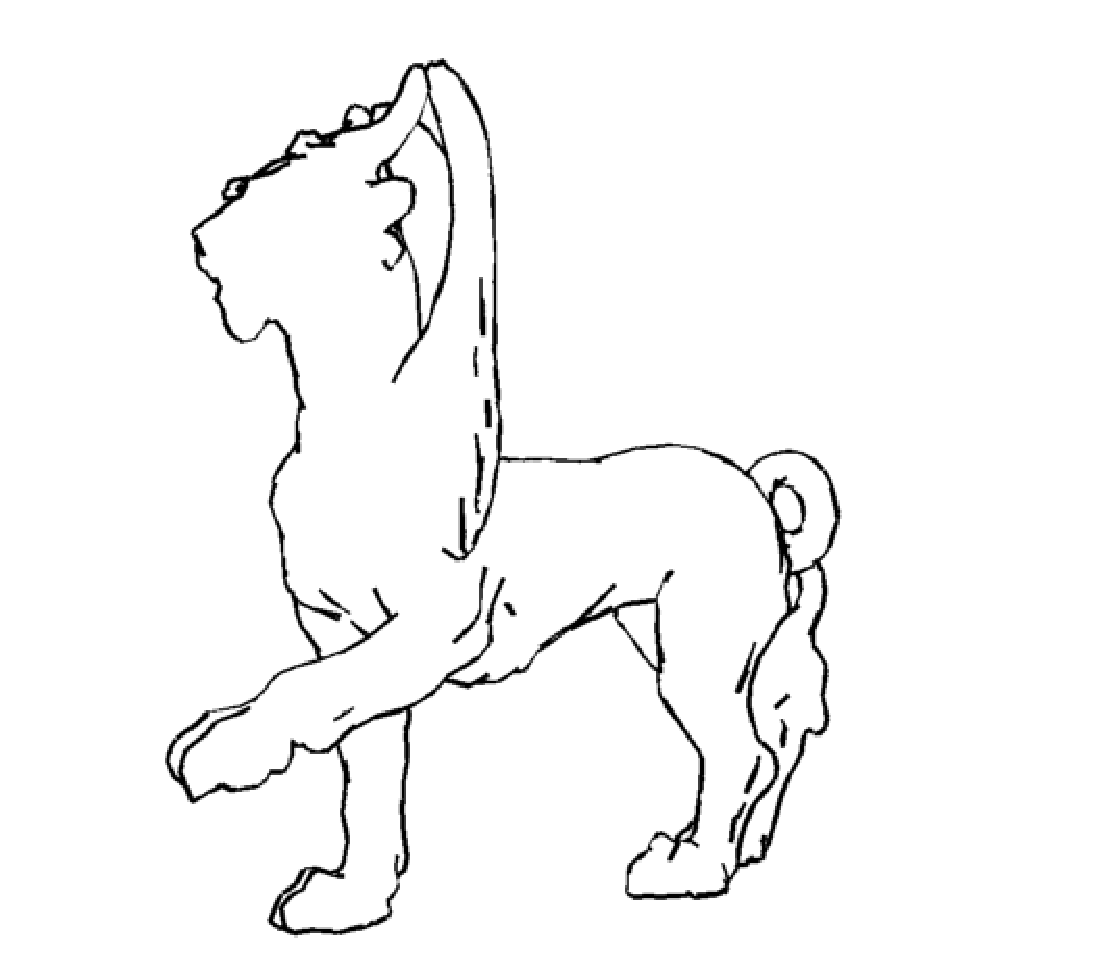
\includegraphics[scale=0.35]{img-2-2/feline-face.eps}}
  \subfloat[vertex-based]{
    \label{fig:vertex-silhouette-feline}
    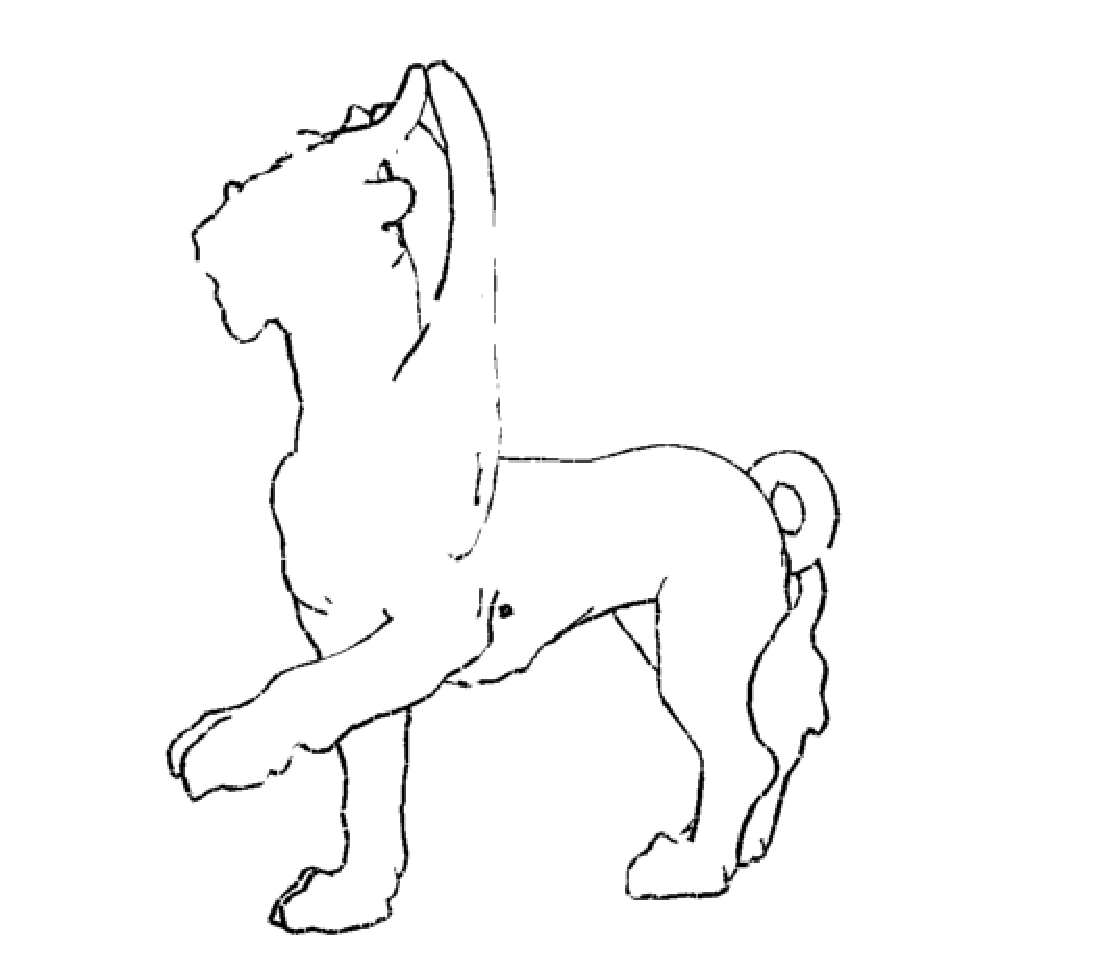
\includegraphics[scale=0.35]{img-2-2/feline-vertex.eps}}
 \caption{Comparison of face- and vertex-based silhouette for the feline}
 \label{fig:silhouette-feline}
\end{figure}

\begin{figure}
  \subfloat[face-based]{
    \label{fig:face-silhouette-buddha}
    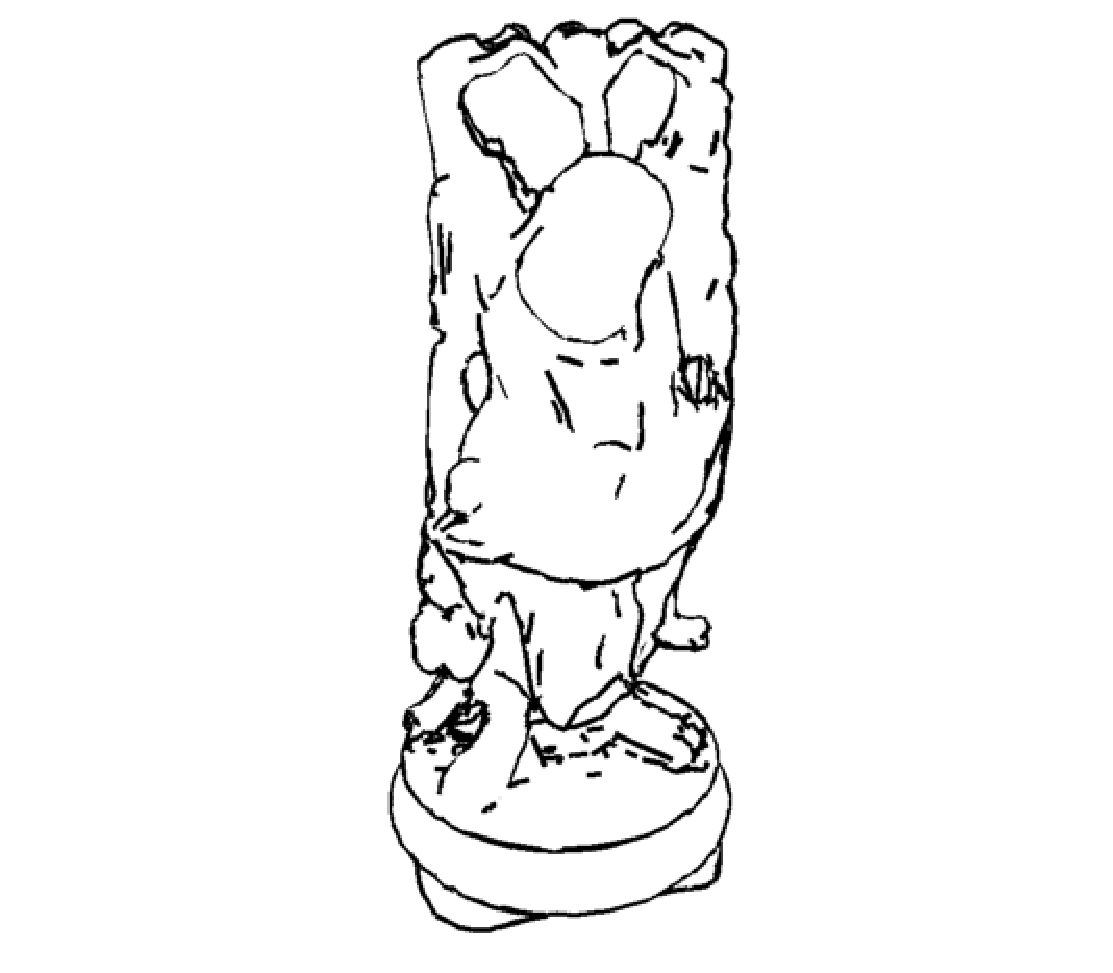
\includegraphics[scale=0.35]{img-2-2/buddha-face.eps}}
  \subfloat[vertex-based]{
    \label{fig:vertex-silhouette-feline}
    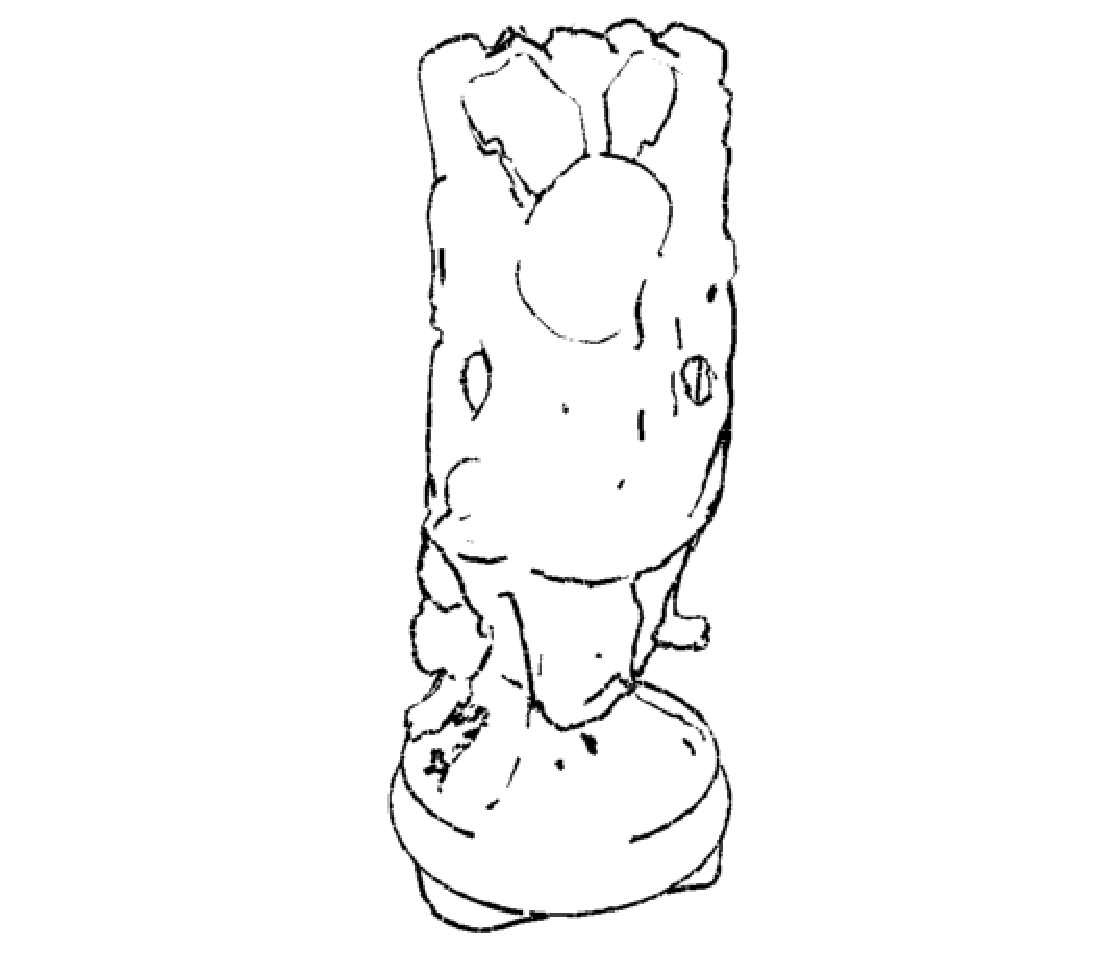
\includegraphics[scale=0.35]{img-2-2/buddha-vertex.eps}}
 \caption{Comparison of face- and vertex-based silhouette for the buddha}
 \label{fig:silhouette-buddha}
\end{figure}

\section{Features}

As I just layed out, the silhouette is only one part of an actual painting,
albeit a very important one. Generally though, an object has other important
features, like e.g. the face of the buddha which is completely bare when viewed
up-front in fig. \ref{fig:silhouette-buddha}. As we learned in class this can
be handled by additionally taking ridges and valleys into account. Especially
the apparent ridges algorithm shown in class should yield good results when
applied to the buddha geometry.

For feature-less objects though, like e.g. the sphere, the ridges and
valleys approach will not yield any good results. Here we should rather apply
an algorithm that takes lightning and curvature into account, like we do later
on in the last exercise.

\section{Silhouette in JavaView}

To actually draw the silhouette in JavaView, one has to add the edges to a
\texttt{PgPolygonSet} using \texttt{addPolygon()}. Furthermore we must prevent
painting of obscured parts of the silhouette, which can be achieved by
keeping the original geometry in the display but coloring its elements
completely white using \texttt{PgElementSet.setGlobalElementColor(Color.white)}
and by disabling lightning via
\texttt{PvDisplayIf.setLightingModel(PvLightIf.MODEL\_SURFACE)}.

\chapter{Curvature estimation}

In the following we are following the steps and algorithms as outlined by Meyer
et al. to estimate the curvature of a discretely triangulated mesh surface. The
code to my implementation can be found in \texttt{Curvature.java} and
\texttt{Ex2\_3.java}.

\section{Curvature Calculation}

The first step is to calculate the mean and gaussian curvature, which can be
done in one go. We iterate over our corner table and for each corner accumulate
the partial addition to the gaussian curvature $\kappa_G$, mean curvature
$\kappa_H$ and area $A_{mixed}$ of the associated vertex. The partial discrete
gaussian curvature is simply the angle $\theta_j$ of the corner, compare to eq.
9 of the paper by Meyer et al. To the mean curvature operator we accumulate
$(\cot \alpha_j + \cot \beta_j) (\vec{x}_i - \vec{x}_j)$, following eq. 8 of the
paper.

Both final curvature values need to be normalized by the area $A_{mixed}$ wich
we also accumulate in each iteration step following fig. 4 of the paper.

Additionally I added the possibility to visualize the minimum and maximum
curvature values using eqs. 10 and 11 from the paper by Meyer et al.

\subsection{Color Schemes}

To visualize the curvature estimations, I developed two simple color schemes.
Both set vertex colors which are then propagated to the triangles using
\texttt{geometry.showElementFromVertexColors(true)}.

Both color schemes leverage the HSV color space with maximum saturation and
value but varying hue component.

\subsubsection{Maximum Color Scheme}

My first approach was to simply map the range $[min, max]$ to the hue range $[0,
360]$, which can be seen in e.g. fig. \ref{fig:bunny-mean-max} or
\ref{fig:bunny-gauss-max}. The minimum value is zero for the mean
curvature and $max$ is the maximum of the computed curvature values. For
gaussian curvature we compute $max = -min$ to be the absolute maximum of the
computed curvature values.

This approach turned out to be a bad choice since the curvature values vary
over a great range. Especially the extreme values are only encountered rarely
though, making the linear mapping between curvature range and hue range
impractical. Due to that this color scheme mostly creates rather equicolored
images.

\subsubsection{Deviation Color Scheme}

To fix the issues of the maximum color scheme, I decided to assume the
curvature to be normal distributed. By calculating the mean value $\mu$ and the
standard deviation $\sigma$ I can now map the curvature values in the tripled
deviation interval $[\mu - 3 \sigma, \mu + 3 \sigma]$ to the hue range $[0,
360]$. This covers $99.73\%$ of the curvature values, the rest is simply capped
to the maximum hue values $0$ or $360$.

This coloring scheme can be seen in e.g. \ref{fig:bunny-mean-dev} and
\ref{fig:bunny-gauss-dev}. Since it gives more useable results, I will
stick to it in the rest of this report.

\begin{figure}
  \subfloat[mean curvature, deviation color scheme]{
    \label{fig:bunny-mean-dev}
    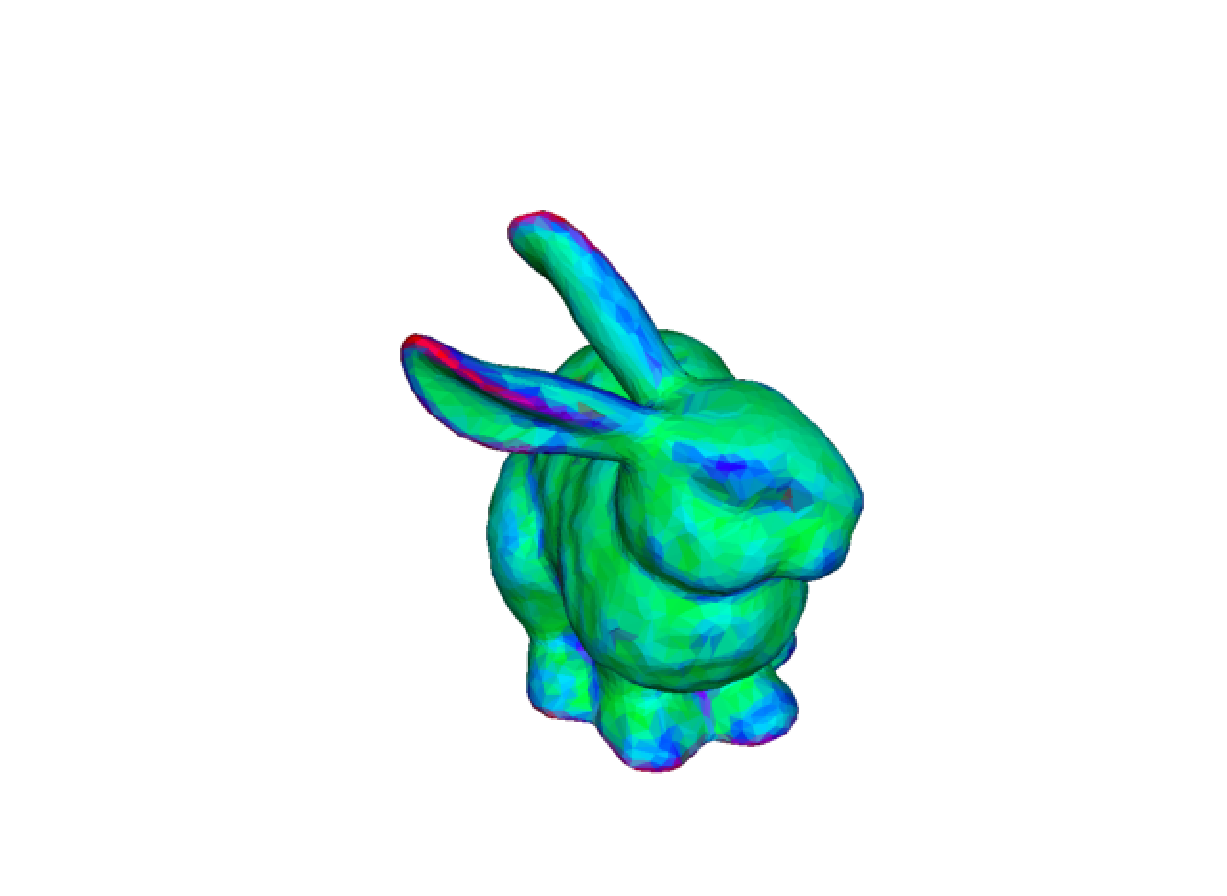
\includegraphics[scale=0.35]{img-2-2/bunny-mean-dev.eps}}
  \subfloat[mean curvature, maximum color scheme]{
    \label{fig:bunny-mean-max}
    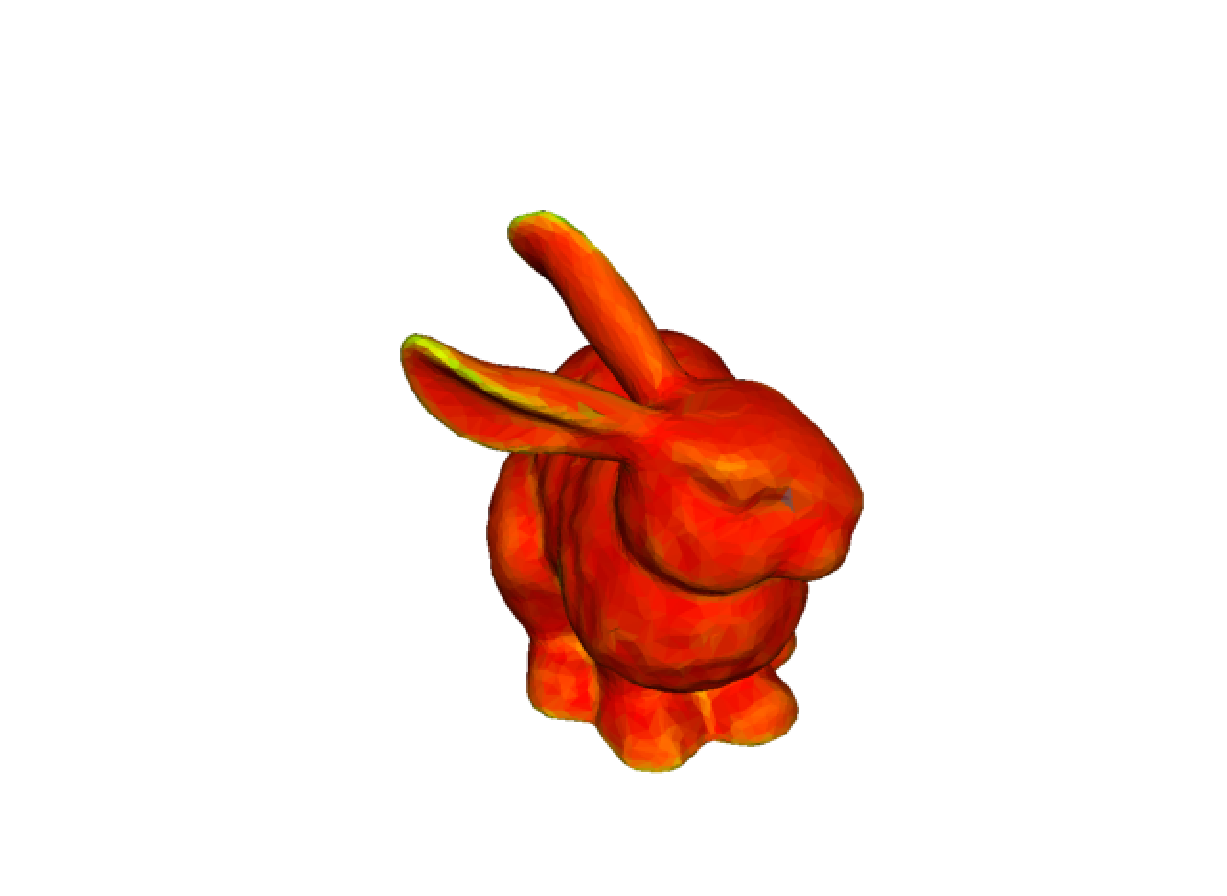
\includegraphics[scale=0.35]{img-2-2/bunny-mean-max.eps}}
  \\
  \subfloat[gaussian curvature, deviation color scheme]{
    \label{fig:bunny-gauss-dev}
    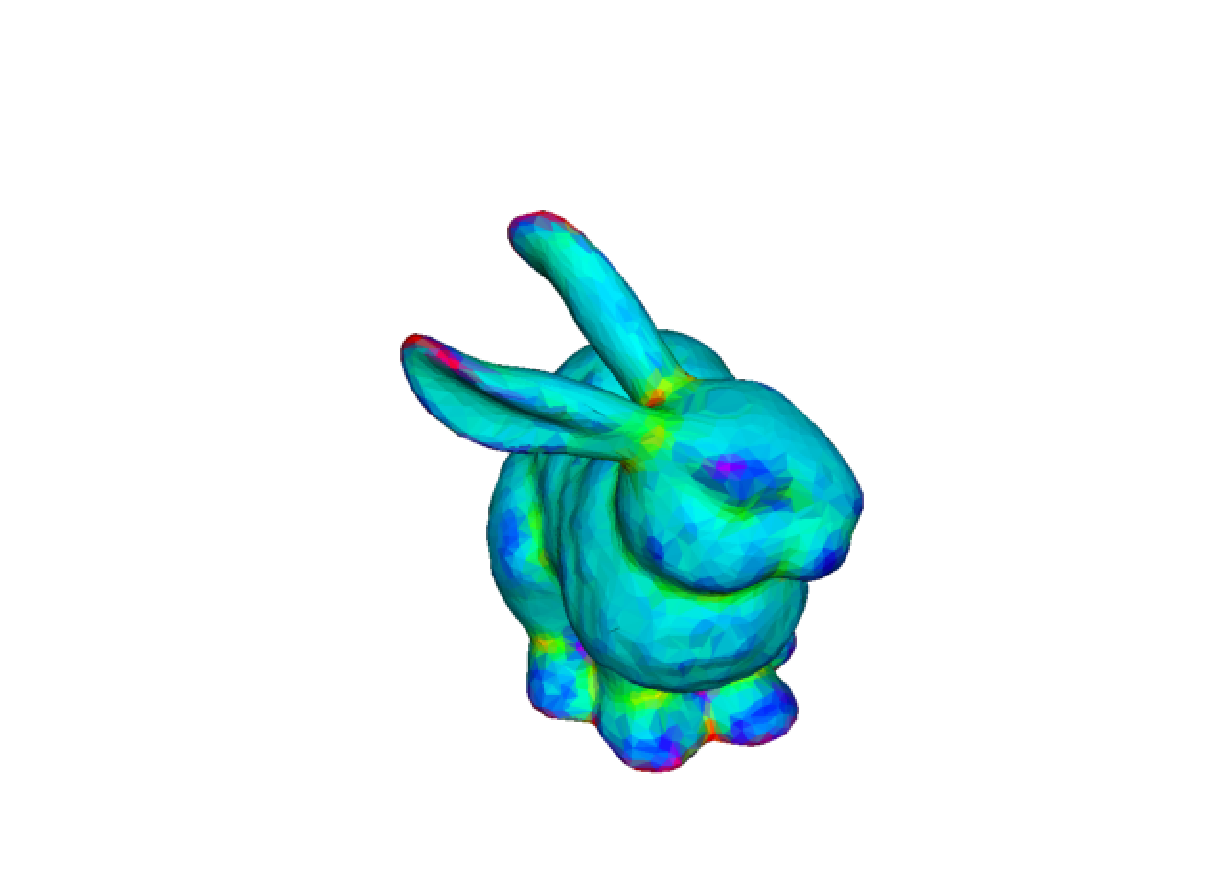
\includegraphics[scale=0.35]{img-2-2/bunny-gauss-dev.eps}}
  \subfloat[gaussian curvature, maximum color scheme]{
    \label{fig:bunny-gauss-max}
    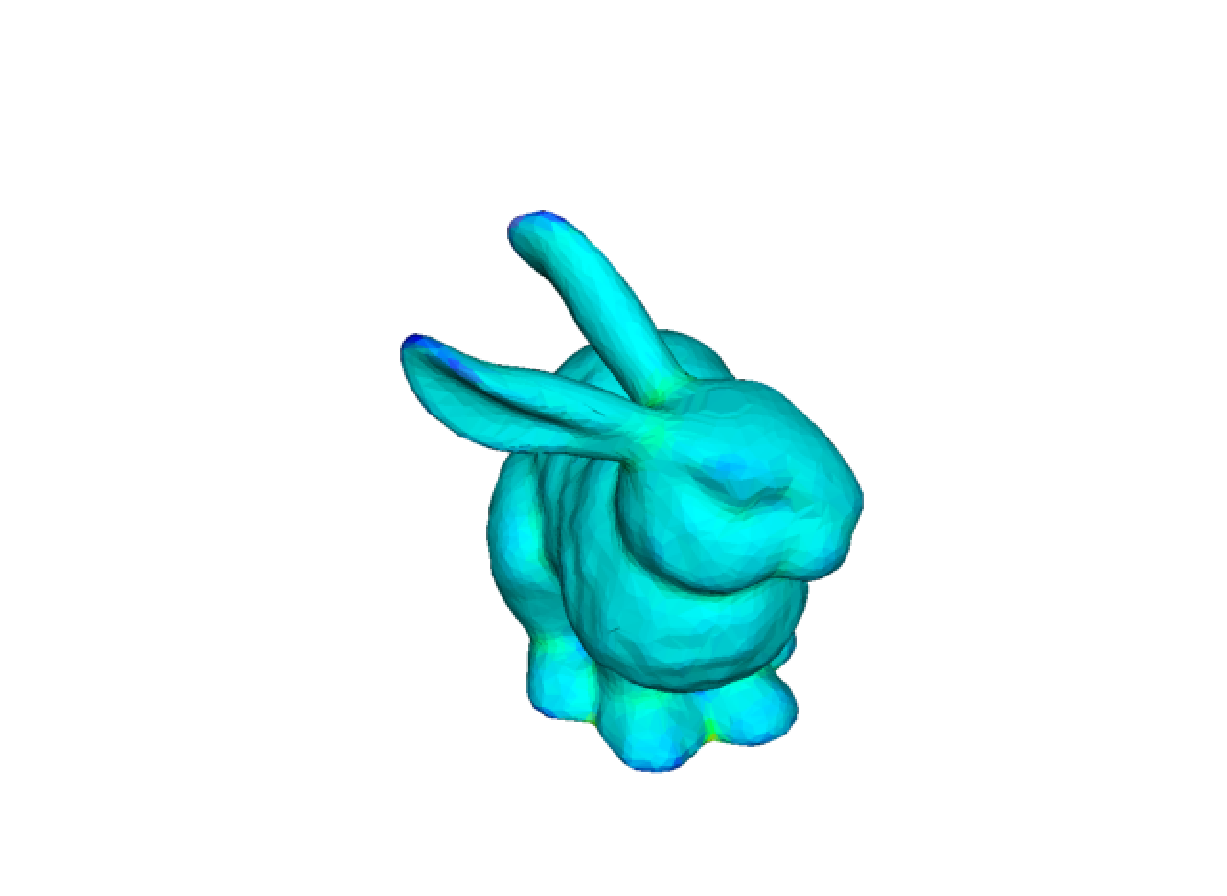
\includegraphics[scale=0.35]{img-2-2/bunny-gauss-max.eps}}
 \caption{Mean and gaussian curvature of the bunny}
 \label{fig:curvature-bunny}
\end{figure}

\subsection{Open Surfaces}

To handled open surfaces like e.g. in fig. \ref{fig:curvature-gauss} somewhat
gracefully, vertices at the edge of a surface are ignored.

\begin{figure}
  \subfloat[mean curvature, deviation color scheme]{
    \label{fig:gauss-mean-dev}
    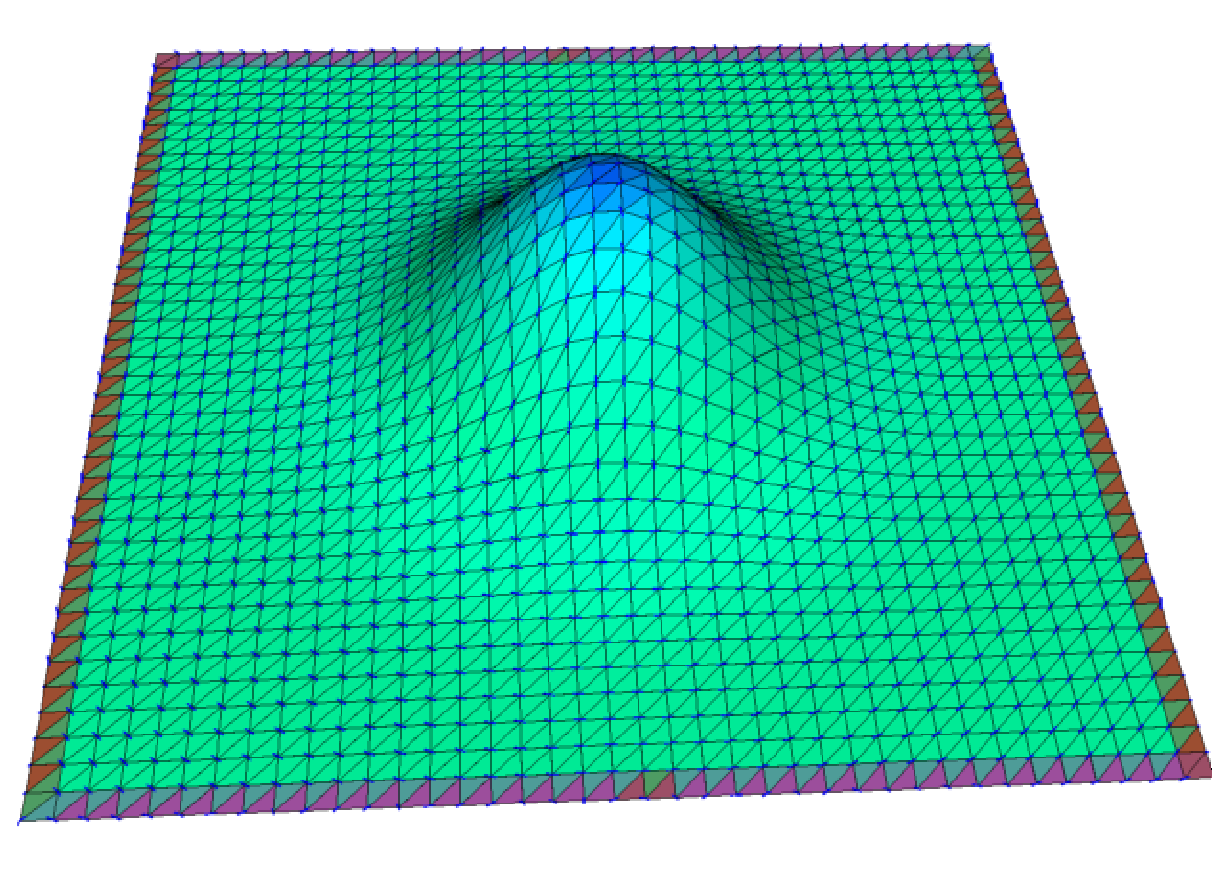
\includegraphics[scale=0.35]{img-2-2/gauss3042-mean-dev.eps}}
  \subfloat[mean curvature, maximum color scheme]{
    \label{fig:gauss-mean-max}
    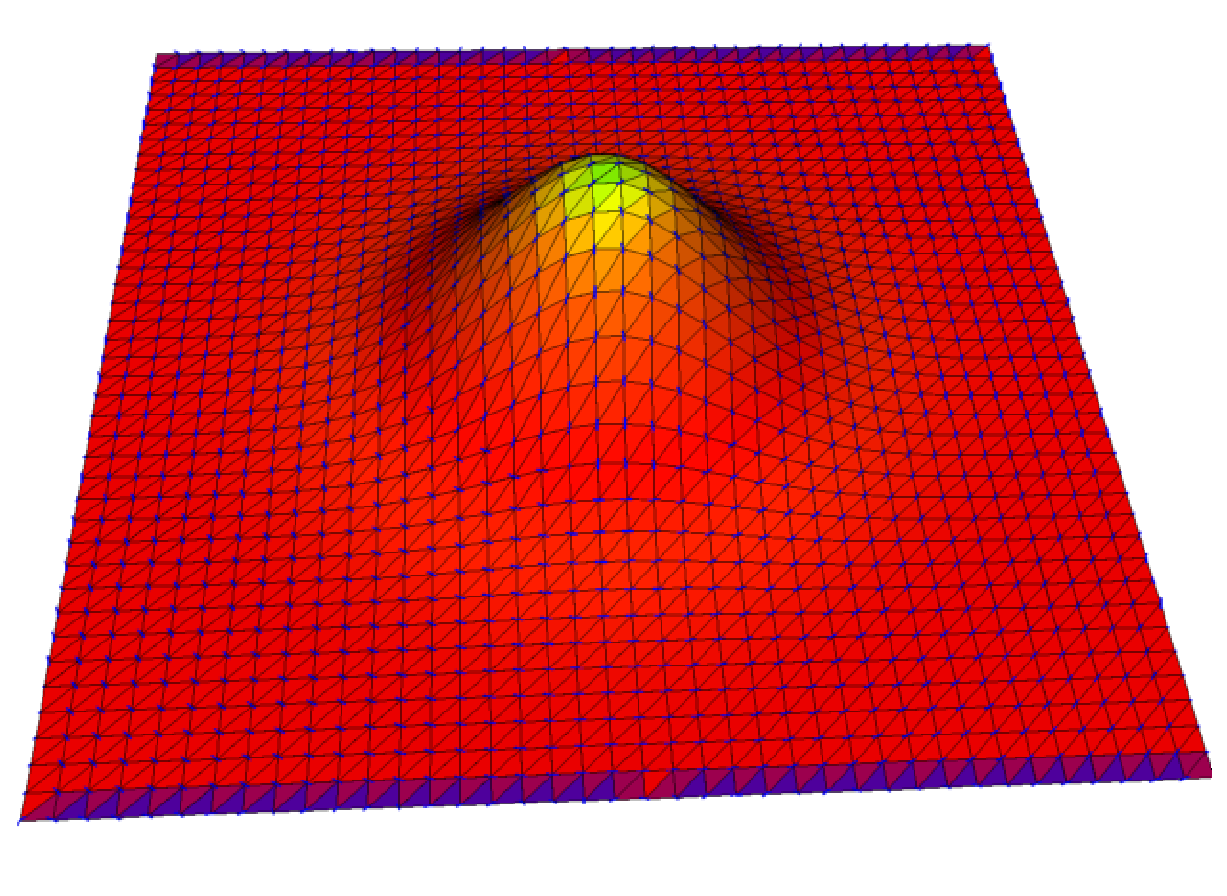
\includegraphics[scale=0.35]{img-2-2/gauss3042-mean-max.eps}}
  \\
  \subfloat[gaussian curvature, deviation color scheme]{
    \label{fig:gauss-gauss-dev}
    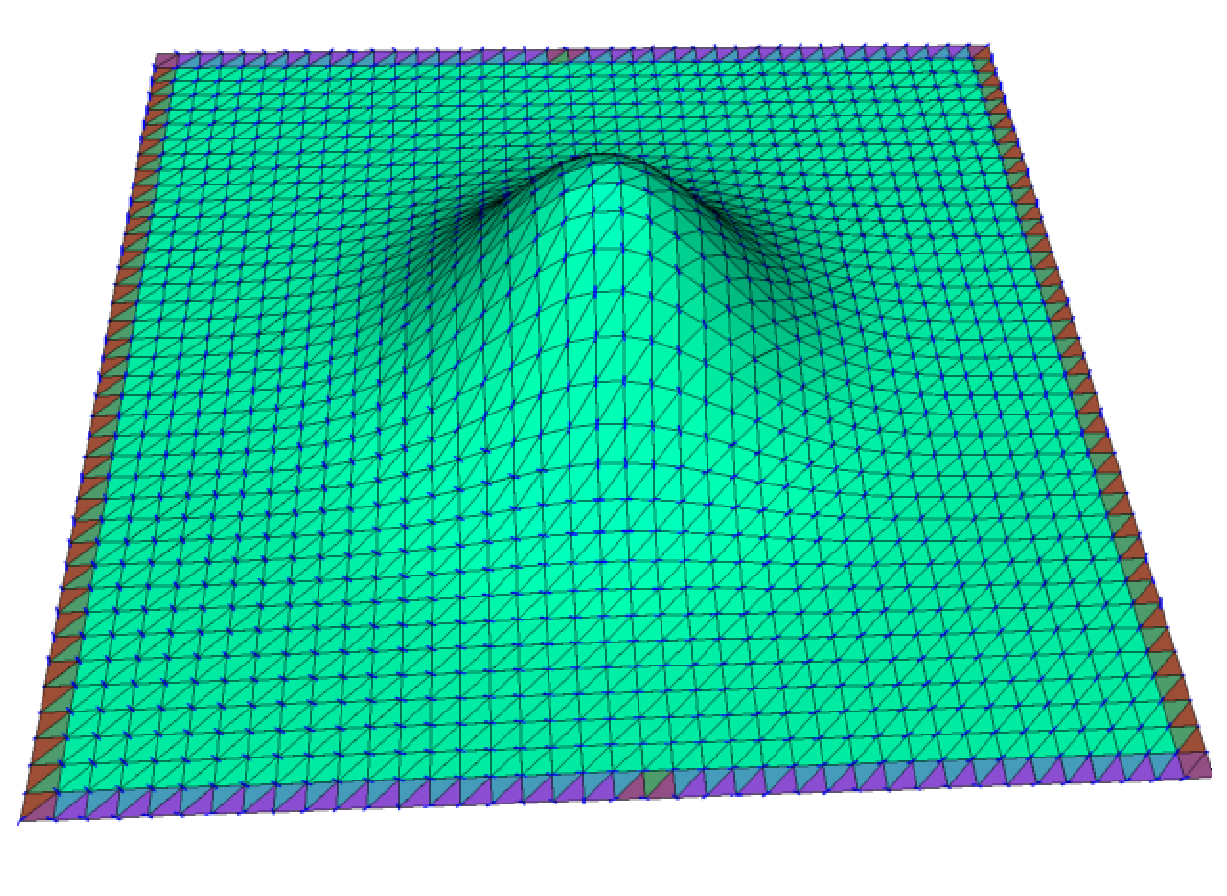
\includegraphics[scale=0.35]{img-2-2/gauss3042-gauss-dev.eps}}
  \subfloat[gaussian curvature, maximum color scheme]{
    \label{fig:gauss-gauss-max}
    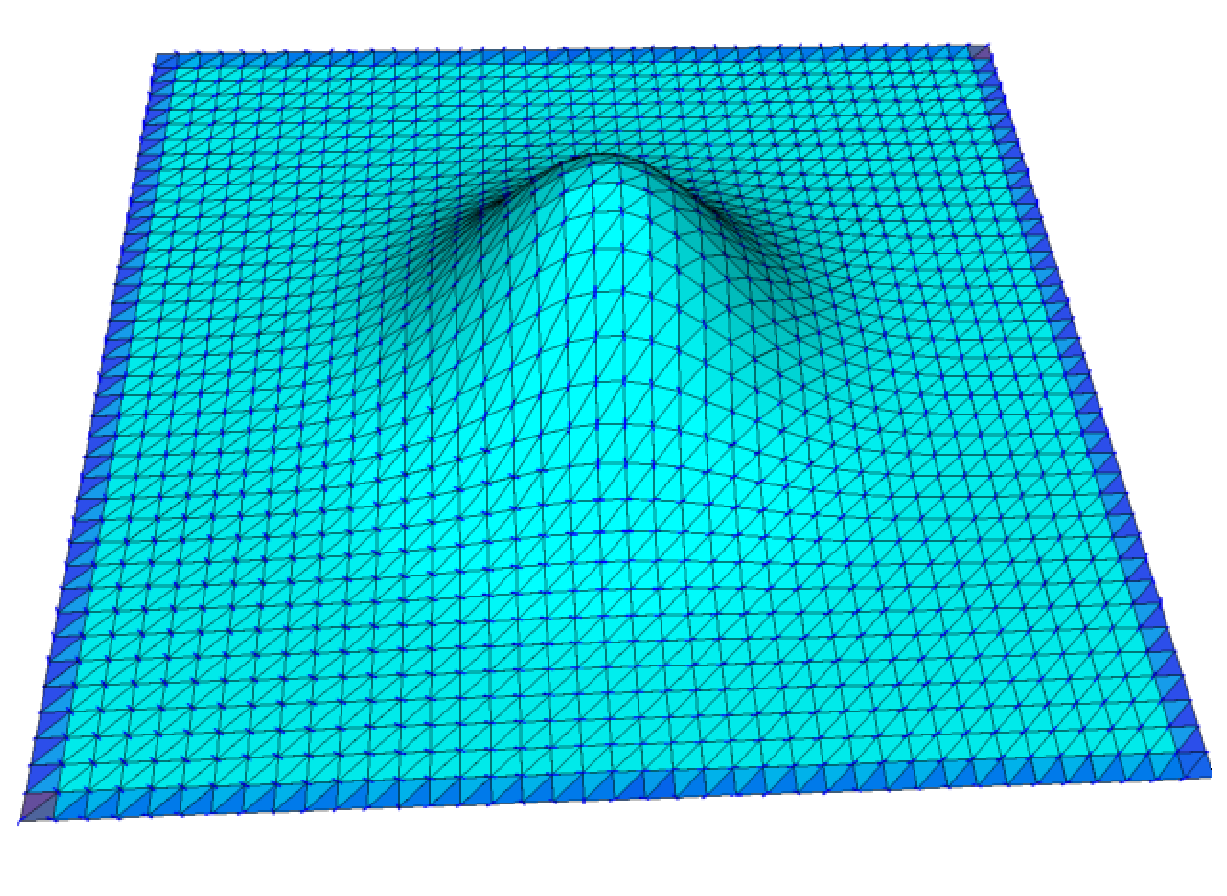
\includegraphics[scale=0.35]{img-2-2/gauss3042-gauss-max.eps}}
 \caption{Mean and gaussian curvature of the \texttt{Gauss\_3042.byu} model with
open surface mesh}
 \label{fig:curvature-gauss}
\end{figure}

\section{Curvature Tensor}

To compute the curvature tensor $\mat{B}$ we iterate over all vertices and
then calculate the $\vec{d}_{i,j}$ values (see p. 14 of the paper by Meyer) for
the 1-ring neighbors using the corner table. This gives us a potentially
over-determined linear equation system in the curvature tensor variables $l$,
$m$, $n$. Following the steps outlined in class 7 (pages 16, 17 of the slides),
we can multiple the eqation system from left with the transposed coefficient
matrix, yielding a square coefficient matrix that can then be solved by
applying Cramer's rule.

While it is quite easily explained, this took me quite some time to implement.
The code can be found in \texttt{Curvature.computeCurvatureTensor()}.

\subsection{Tensor Visualization}

To visualize the curvature tensor, we compute the principle directions of it,
i.e. the two dimensional eigen vectors $\vec{e}_{minor}$ and $\vec{e}_{major}$.
These are easily mapped to three dimensions by blending the three dimensional
tangent plane vectors $x$, $y$ by the associated value of each eigen vector.

These vectors can then be added to a \texttt{PgVectorField} in JavaView with a
user defined length to visualize the curvature tensor.

A few results can be seen in \ref{fig:curvature-tensor}, the code to my
implementation can be found in
\texttt{Curvature.computeCurvatureTensorFields()}.

\begin{figure}
  \subfloat[minor]{
    \label{fig:dragon-t-minor}
    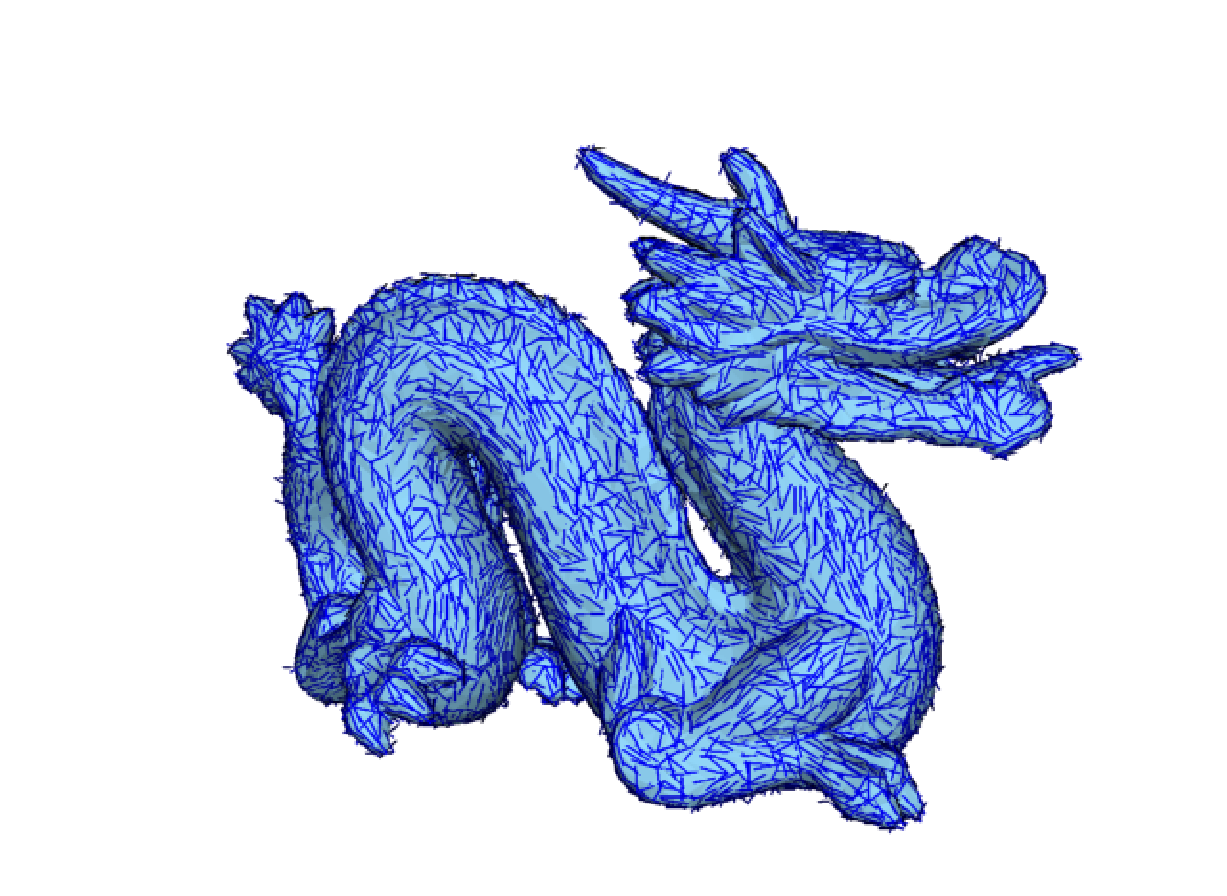
\includegraphics[scale=0.35]{img-2-2/dragon-t-minor.eps}}
  \subfloat[major]{
    \label{fig:dragon-t-major}
    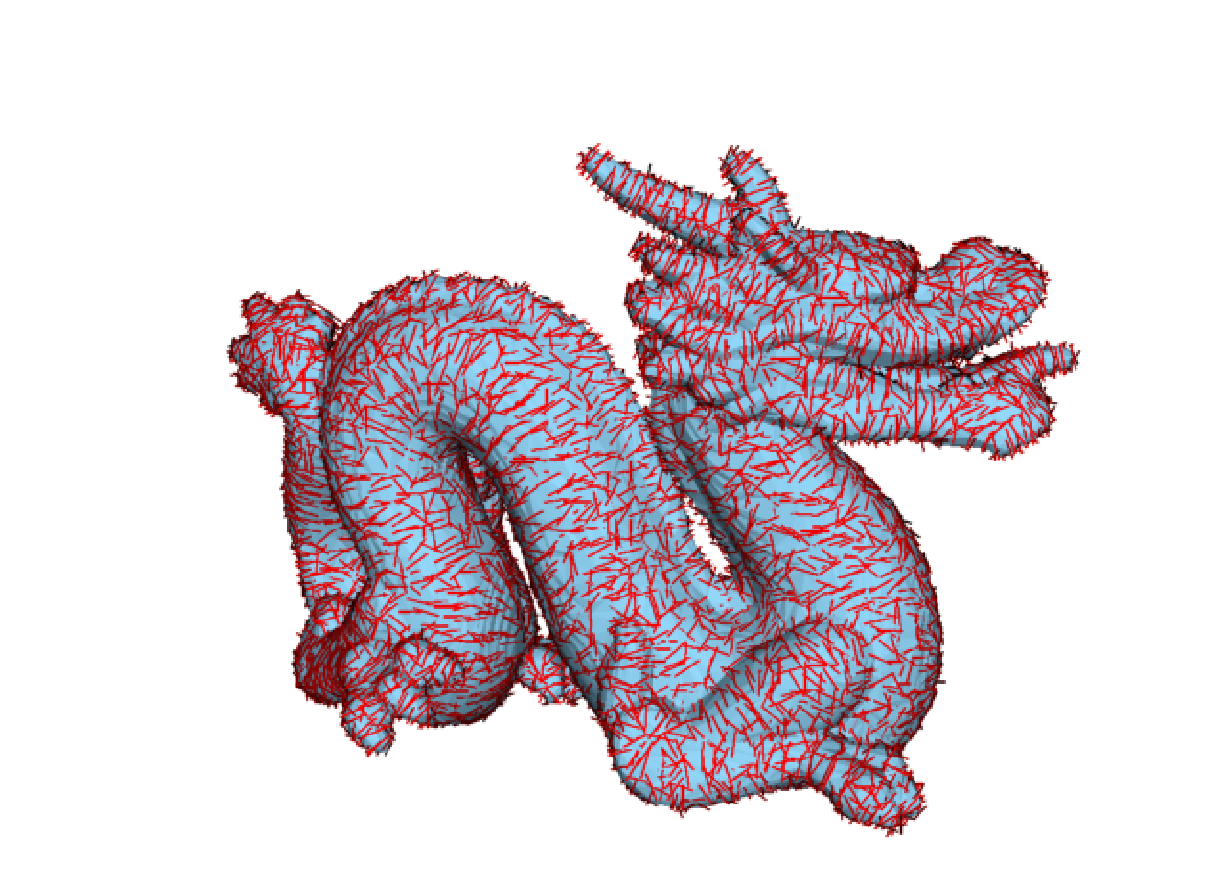
\includegraphics[scale=0.35]{img-2-2/dragon-t-major.eps}}
  \\
  \subfloat[minor]{
    \label{fig:feline-t-minor}
    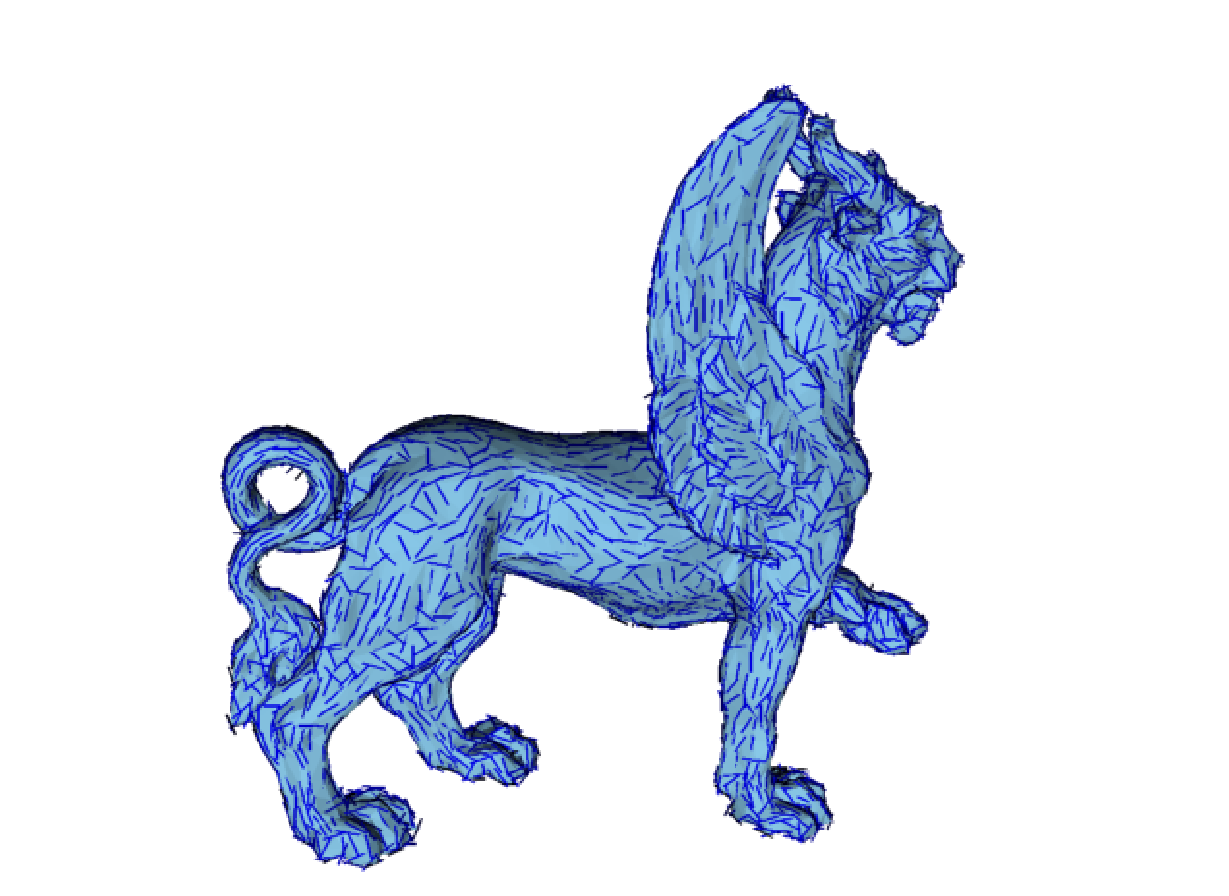
\includegraphics[scale=0.35]{img-2-2/feline-t-minor.eps}}
  \subfloat[major]{
    \label{fig:feline-t-major}
    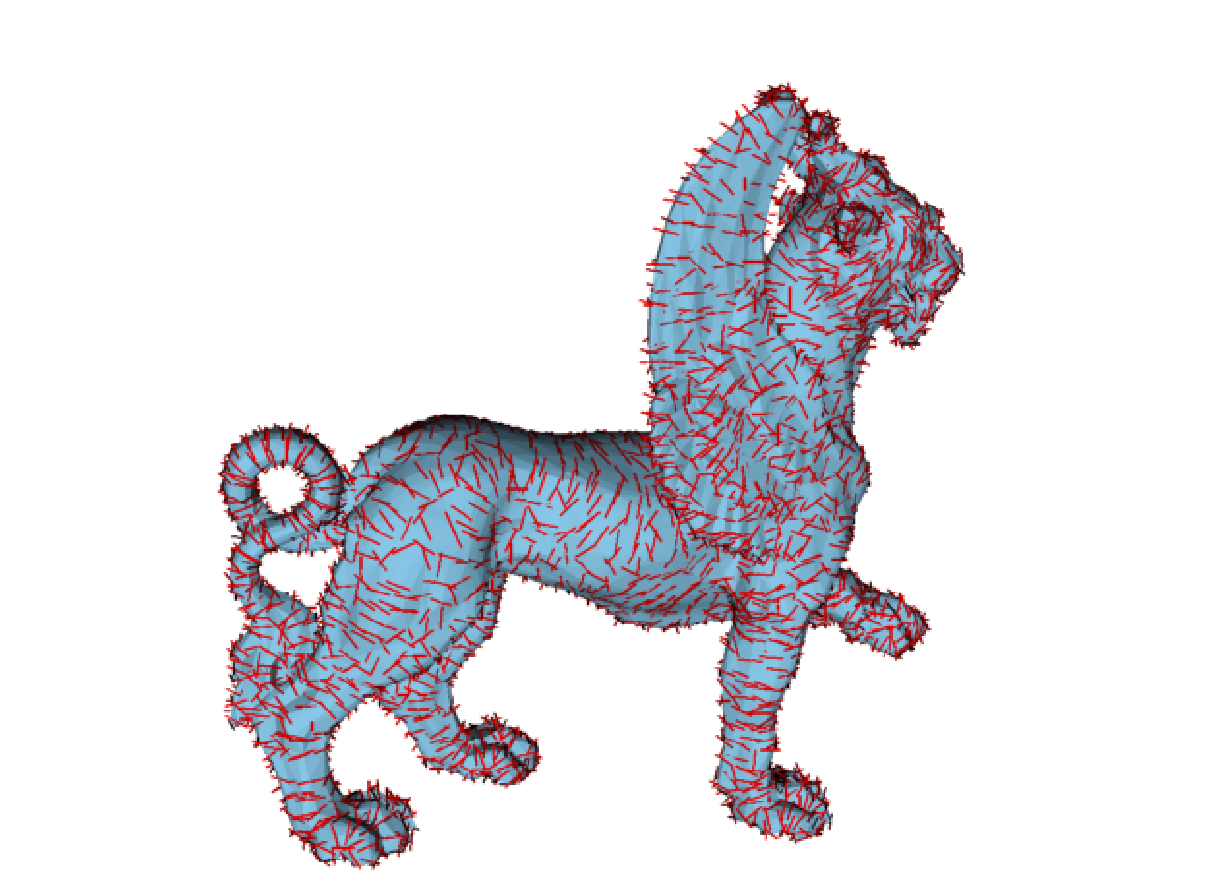
\includegraphics[scale=0.35]{img-2-2/feline-t-major.eps}}
  \\
  \subfloat[minor]{
    \label{fig:torus-t-minor}
    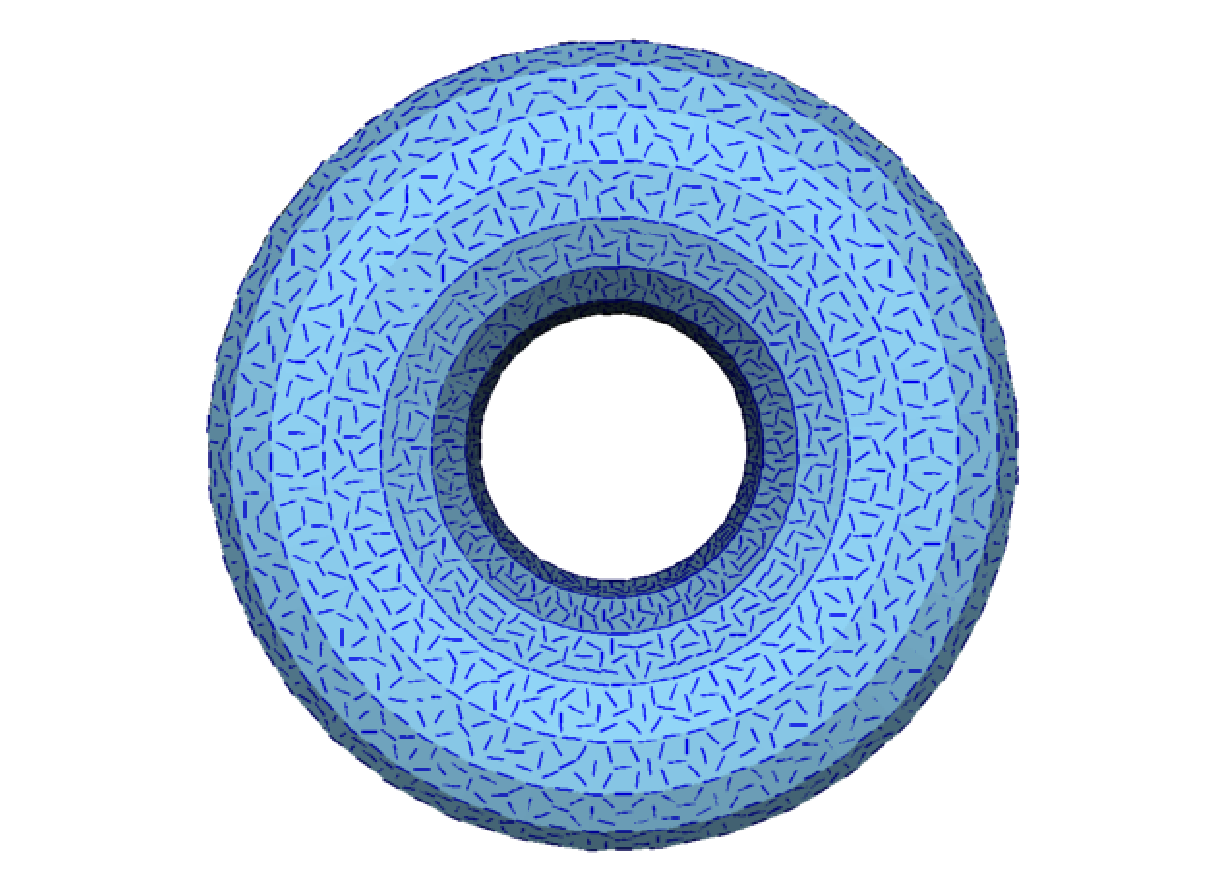
\includegraphics[scale=0.35]{img-2-2/torus-t-minor.eps}}
  \subfloat[major]{
    \label{fig:torus-t-major}
    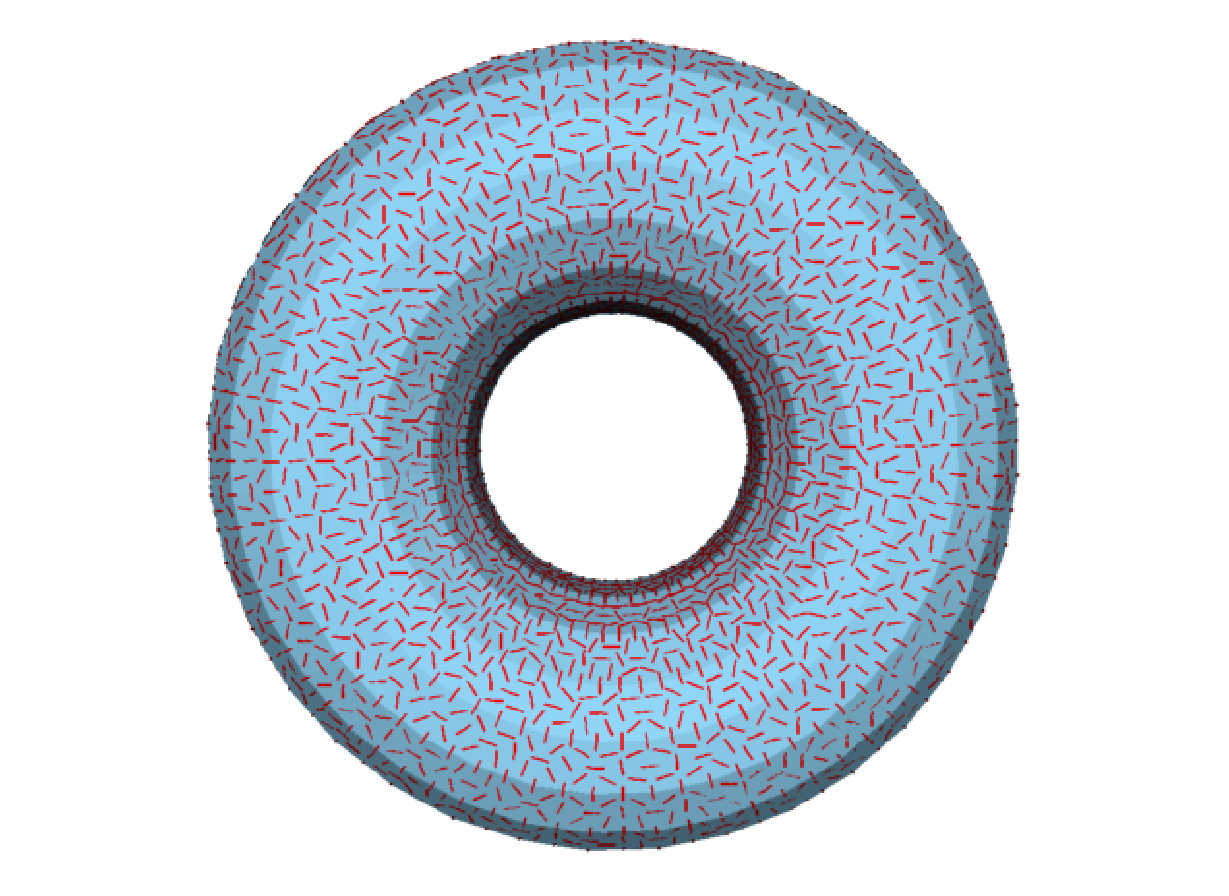
\includegraphics[scale=0.35]{img-2-2/torus-t-major.eps}}
 \caption{Minor and Major principle directions of the curvature tensor}
 \label{fig:curvature-tensor}
\end{figure}

\section{Total Angle Deficit}

The sum of the angles $\theta_{i,j}$ turns out to always be an integral multiple
of $2 \pi$. And indeed I find $N - \sum_{i,j} \theta_{i,j} = \chi$, with $N$
being the total number of vertices in the geometry and $\chi$ the euler
characteristic of the geometry.

This does not work for geometries with curvature singularities
though, like e.g. the hand. There the angle deficit will be
improperly calculated and hence does not map to the euler
characteristic anylonger.

To verify this, run \texttt{Ex2\_3.java} on a selected geometry. The total angle
deficit and euler characteristic will be outputted to the console.

\section{Tensor Smoothing}

As seen in fig. \ref{fig:curvature-tensor}, the raw curvature tensor is rather
noisy. For a more visually pleasing image, we must smoothen it.

To do this we first scale the local $2x2$ curvature tensor into the global
$3x3$ frame, following the steps outlined in class and in the recitation. The
source code for this can be found in $VertexCurvature.globalCurvature()$.

Now we can smoothen the tensors using either the explicit or forward-Euler
scheme or the Gauss-Seidel scheme. Both can be run for a user-defined number of
times with a user-defined step size. Furthermore we can apply different
weights, either uniform, cord, cotangent or mean value based. See the slides to
class 9 for details.

My implementation can be found in \texttt{Ex2\_3.java} and
\texttt{Curvature.smoothTensorField()}.

\subsection{Weighting Comparison}

To compare the weighting types, see e.g. fig.
\ref{fig:smooth-weights-curvature-tensor}.

\subsection{Uniform}

The uniform weighting is fast and gives reasonable results.

\subsection{Cord}

Weighting the tensors by the reziproke edge distance turns out to give worse
results compared to the uniform weighting.

\subsection{Mean Value}

Weighting the tensors by mean value gives better results than the cord
weighting, yet interestingly enough does not seem to be as effective as the
uniform weighting. It is also noticeably slower for large geometries or number
of steps.

\subsection{Cotangent}

The cotangent weighting yields comparable results to the mean value approach.

\begin{figure}
  \subfloat[uniform]{
    \label{fig:dragon-t-10-01-uniform}
   
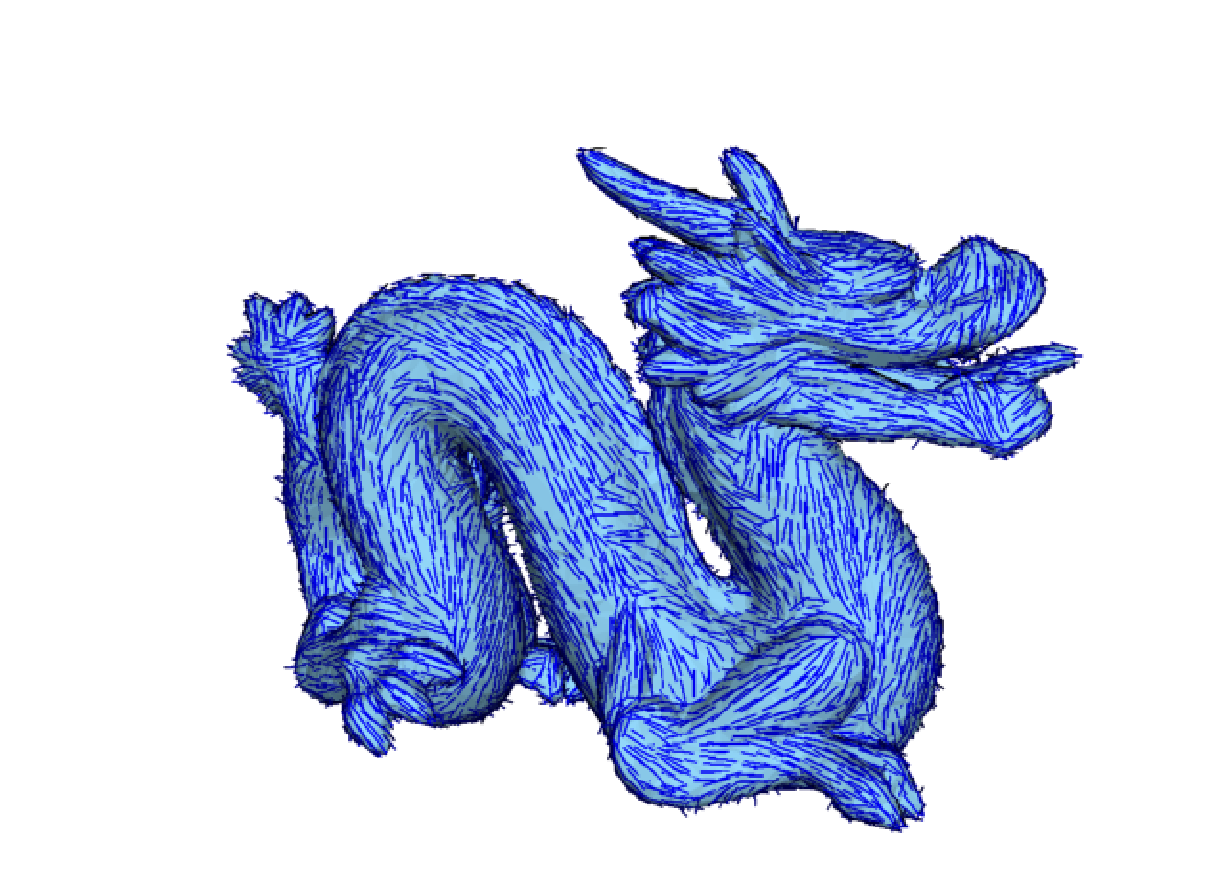
\includegraphics[scale=0.35]{img-2-2/dragon-t-10-01-uniform-forwardeuler.eps}}
  \subfloat[cord]{
    \label{fig:dragon-t-10-01-cord}
    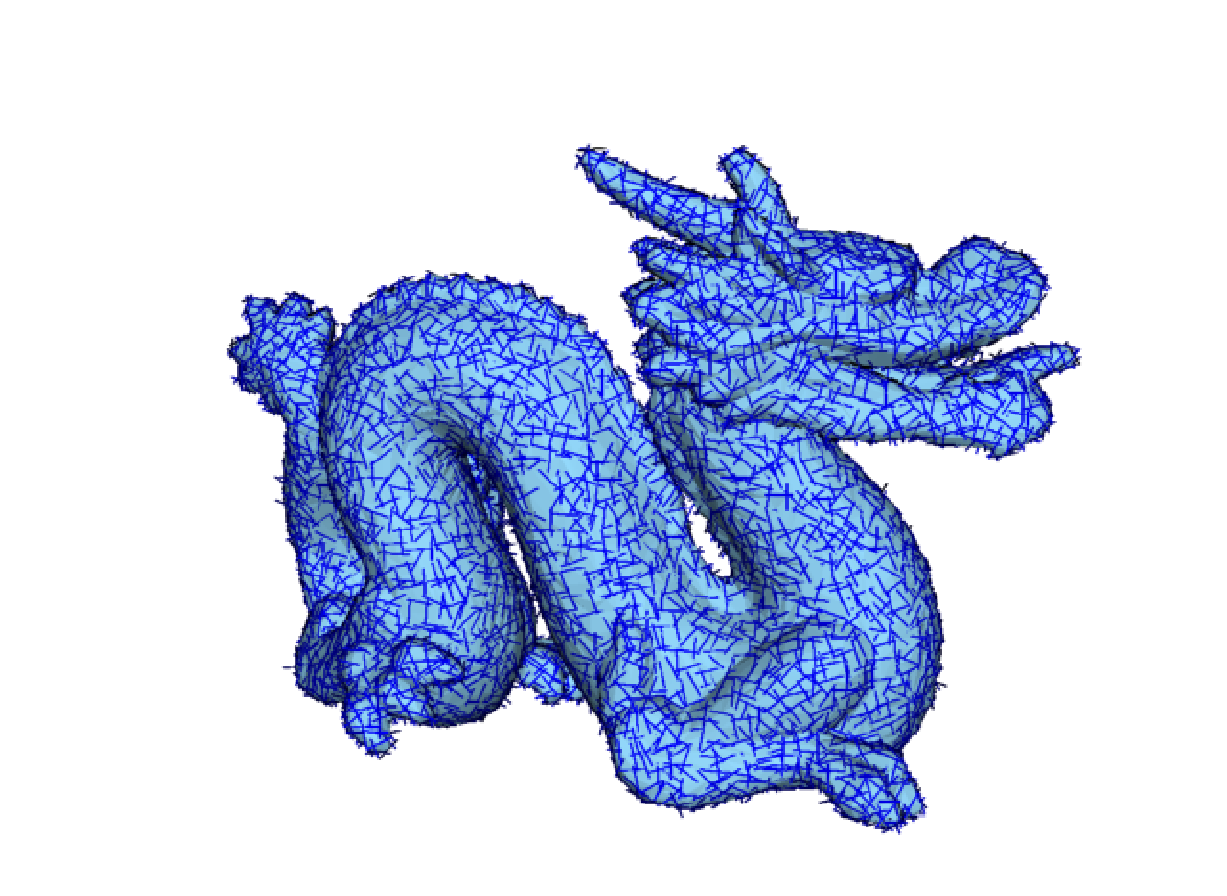
\includegraphics[scale=0.35]{img-2-2/dragon-t-10-01-cord-forwardeuler.eps}}
  \\
  \subfloat[mean]{
    \label{fig:dragon-t-10-01-mean}
    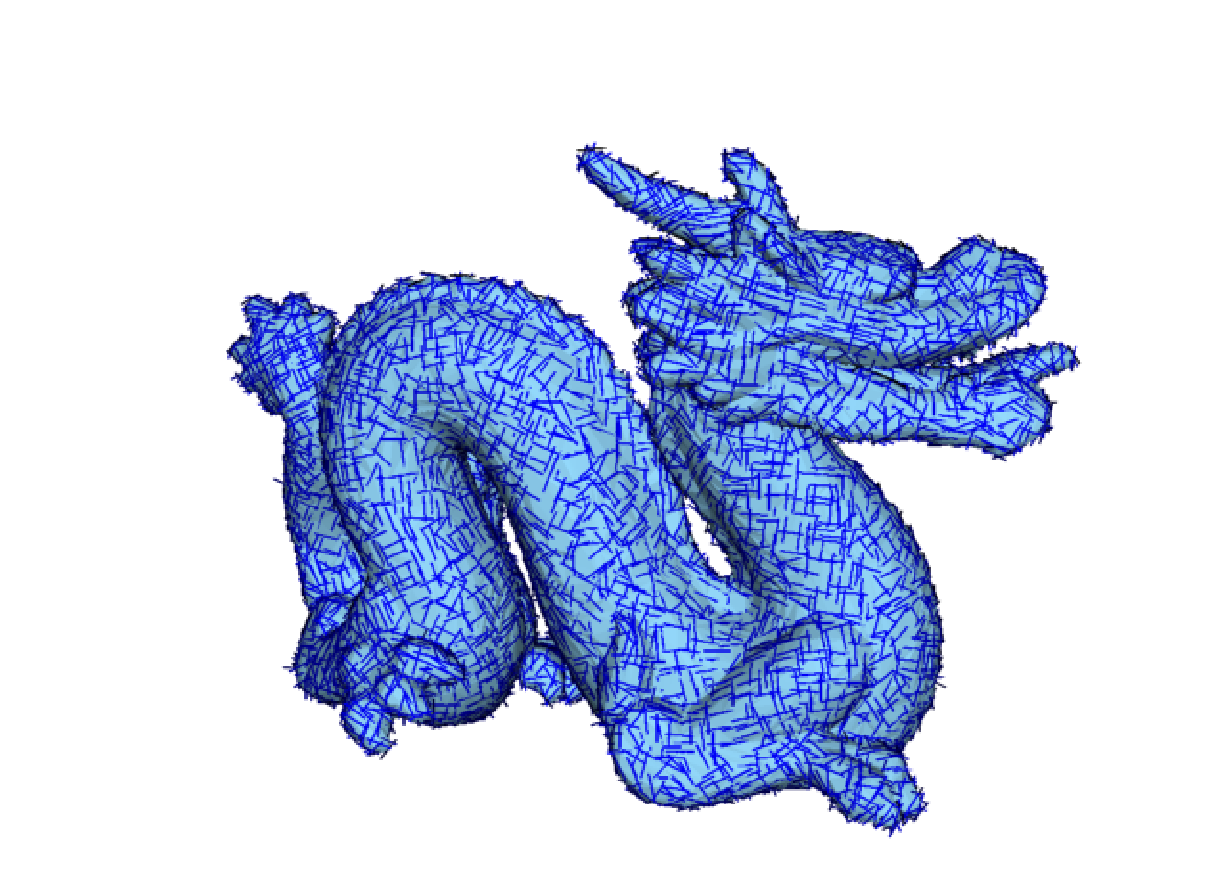
\includegraphics[scale=0.35]{img-2-2/dragon-t-10-01-mean-forwardeuler.eps}}
  \subfloat[cotangent]{
    \label{fig:dragon-t-10-01-cotangent}
    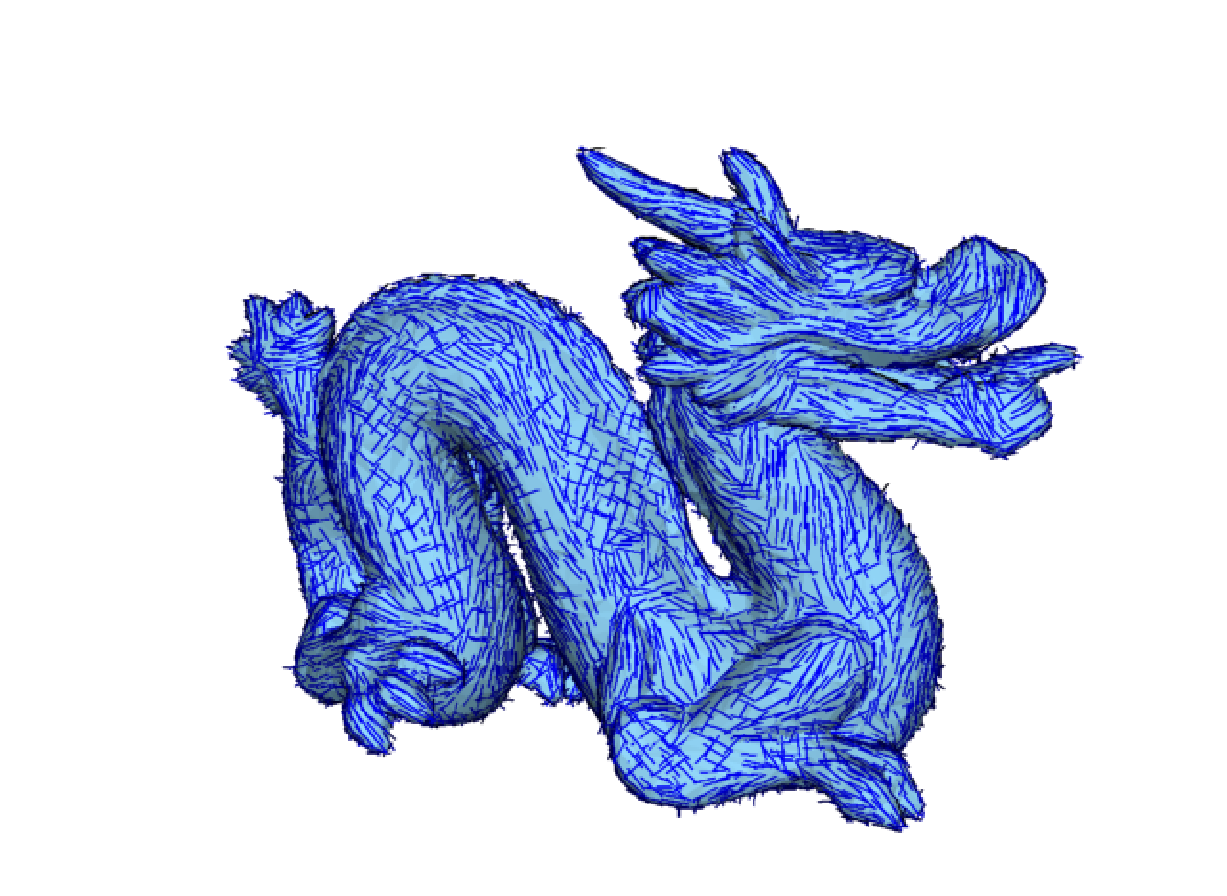
\includegraphics[scale=0.35]{img-2-2/dragon-t-10-01-cotan-forwardeuler.eps}}
 \caption{smoothened tensor field of the dragon using different weights: steps:
10, step size: $0.1$, scheme: forward-euler}
 \label{fig:smooth-weights-curvature-tensor}
\end{figure}


\end{document}

% kate: replace-tabs on;